\documentclass[twoside]{book}

% Packages required by doxygen
\usepackage{fixltx2e}
\usepackage{calc}
\usepackage{doxygen}
\usepackage[export]{adjustbox} % also loads graphicx
\usepackage{graphicx}
\usepackage[utf8]{inputenc}
\usepackage{makeidx}
\usepackage{multicol}
\usepackage{multirow}
\PassOptionsToPackage{warn}{textcomp}
\usepackage{textcomp}
\usepackage[nointegrals]{wasysym}
\usepackage[table]{xcolor}

% Font selection
\usepackage[T1]{fontenc}
\usepackage[scaled=.90]{helvet}
\usepackage{courier}
\usepackage{amssymb}
\usepackage{sectsty}
\renewcommand{\familydefault}{\sfdefault}
\allsectionsfont{%
  \fontseries{bc}\selectfont%
  \color{darkgray}%
}
\renewcommand{\DoxyLabelFont}{%
  \fontseries{bc}\selectfont%
  \color{darkgray}%
}
\newcommand{\+}{\discretionary{\mbox{\scriptsize$\hookleftarrow$}}{}{}}

% Page & text layout
\usepackage{geometry}
\geometry{%
  a4paper,%
  top=2.5cm,%
  bottom=2.5cm,%
  left=2.5cm,%
  right=2.5cm%
}
\tolerance=750
\hfuzz=15pt
\hbadness=750
\setlength{\emergencystretch}{15pt}
\setlength{\parindent}{0cm}
\setlength{\parskip}{3ex plus 2ex minus 2ex}
\makeatletter
\renewcommand{\paragraph}{%
  \@startsection{paragraph}{4}{0ex}{-1.0ex}{1.0ex}{%
    \normalfont\normalsize\bfseries\SS@parafont%
  }%
}
\renewcommand{\subparagraph}{%
  \@startsection{subparagraph}{5}{0ex}{-1.0ex}{1.0ex}{%
    \normalfont\normalsize\bfseries\SS@subparafont%
  }%
}
\makeatother

% Headers & footers
\usepackage{fancyhdr}
\pagestyle{fancyplain}
\fancyhead[LE]{\fancyplain{}{\bfseries\thepage}}
\fancyhead[CE]{\fancyplain{}{}}
\fancyhead[RE]{\fancyplain{}{\bfseries\leftmark}}
\fancyhead[LO]{\fancyplain{}{\bfseries\rightmark}}
\fancyhead[CO]{\fancyplain{}{}}
\fancyhead[RO]{\fancyplain{}{\bfseries\thepage}}
\fancyfoot[LE]{\fancyplain{}{}}
\fancyfoot[CE]{\fancyplain{}{}}
\fancyfoot[RE]{\fancyplain{}{\bfseries\scriptsize Generated by Doxygen }}
\fancyfoot[LO]{\fancyplain{}{\bfseries\scriptsize Generated by Doxygen }}
\fancyfoot[CO]{\fancyplain{}{}}
\fancyfoot[RO]{\fancyplain{}{}}
\renewcommand{\footrulewidth}{0.4pt}
\renewcommand{\chaptermark}[1]{%
  \markboth{#1}{}%
}
\renewcommand{\sectionmark}[1]{%
  \markright{\thesection\ #1}%
}

% Indices & bibliography
\usepackage{natbib}
\usepackage[titles]{tocloft}
\setcounter{tocdepth}{3}
\setcounter{secnumdepth}{5}
\makeindex

% Hyperlinks (required, but should be loaded last)
\usepackage{ifpdf}
\ifpdf
  \usepackage[pdftex,pagebackref=true]{hyperref}
\else
  \usepackage[ps2pdf,pagebackref=true]{hyperref}
\fi
\hypersetup{%
  colorlinks=true,%
  linkcolor=blue,%
  citecolor=blue,%
  unicode%
}

% Custom commands
\newcommand{\clearemptydoublepage}{%
  \newpage{\pagestyle{empty}\cleardoublepage}%
}

\usepackage{caption}
\captionsetup{labelsep=space,justification=centering,font={bf},singlelinecheck=off,skip=4pt,position=top}

%===== C O N T E N T S =====

\begin{document}

% Titlepage & ToC
\hypersetup{pageanchor=false,
             bookmarksnumbered=true,
             pdfencoding=unicode
            }
\pagenumbering{roman}
\begin{titlepage}
\vspace*{7cm}
\begin{center}%
{\Large vinecopulib \\[1ex]\large 0.\+0.\+1.\+9990 }\\
\vspace*{1cm}
{\large Generated by Doxygen 1.8.11}\\
\end{center}
\end{titlepage}
\clearemptydoublepage
\tableofcontents
\clearemptydoublepage
\pagenumbering{arabic}
\hypersetup{pageanchor=true}

%--- Begin generated contents ---
\chapter{vinecopulib\+: a C++ library for vine copula modeling}
\label{index}\hypertarget{index}{}\begin{DoxyAuthor}{Authors}
Thomas Nagler and Thibault Vatter
\end{DoxyAuthor}
This is the A\+PI documentation for the vinecopulib C++ library. It provides functionality for statistical dependence modeling with bivariate and vine copulas. For a more high-\/level overview see \href{https://github.com/tvatter/vinecopulib/blob/master/README.md}{\tt R\+E\+A\+D\+ME}.\hypertarget{index_license}{}\section{License}\label{index_license}
The M\+IT License (M\+IT)

Copyright © 2017 Thibault Vatter and Thomas Nagler

Permission is hereby granted, free of charge, to any person obtaining a copy of this software and associated documentation files (the “\+Software”), to deal in the Software without restriction, including without limitation the rights to use, copy, modify, merge, publish, distribute, sublicense, and/or sell copies of the Software, and to permit persons to whom the Software is furnished to do so, subject to the following conditions\+:

The above copyright notice and this permission notice shall be included in all copies or substantial portions of the Software.

T\+HE S\+O\+F\+T\+W\+A\+RE IS P\+R\+O\+V\+I\+D\+ED “\+AS I\+S”, W\+I\+T\+H\+O\+UT W\+A\+R\+R\+A\+N\+TY OF A\+NY K\+I\+ND, E\+X\+P\+R\+E\+SS OR I\+M\+P\+L\+I\+ED, I\+N\+C\+L\+U\+D\+I\+NG B\+UT N\+OT L\+I\+M\+I\+T\+ED TO T\+HE W\+A\+R\+R\+A\+N\+T\+I\+ES OF M\+E\+R\+C\+H\+A\+N\+T\+A\+B\+I\+L\+I\+TY, F\+I\+T\+N\+E\+SS F\+OR A P\+A\+R\+T\+I\+C\+U\+L\+AR P\+U\+R\+P\+O\+SE A\+ND N\+O\+N\+I\+N\+F\+R\+I\+N\+G\+E\+M\+E\+NT. IN NO E\+V\+E\+NT S\+H\+A\+LL T\+HE A\+U\+T\+H\+O\+RS OR C\+O\+P\+Y\+R\+I\+G\+HT H\+O\+L\+D\+E\+RS BE L\+I\+A\+B\+LE F\+OR A\+NY C\+L\+A\+IM, D\+A\+M\+A\+G\+ES OR O\+T\+H\+ER L\+I\+A\+B\+I\+L\+I\+TY, W\+H\+E\+T\+H\+ER IN AN A\+C\+T\+I\+ON OF C\+O\+N\+T\+R\+A\+CT, T\+O\+RT OR O\+T\+H\+E\+R\+W\+I\+SE, A\+R\+I\+S\+I\+NG F\+R\+OM, O\+UT OF OR IN C\+O\+N\+N\+E\+C\+T\+I\+ON W\+I\+TH T\+HE S\+O\+F\+T\+W\+A\+RE OR T\+HE U\+SE OR O\+T\+H\+ER D\+E\+A\+L\+I\+N\+GS IN T\+HE S\+O\+F\+T\+W\+A\+RE. 
\chapter{Module Index}
\section{Modules}
Here is a list of all modules\+:\begin{DoxyCompactList}
\item \contentsline{section}{Readers}{\pageref{group__readers}}{}
\end{DoxyCompactList}

\chapter{Hierarchical Index}
\section{Class Hierarchy}
This inheritance list is sorted roughly, but not completely, alphabetically\+:\begin{DoxyCompactList}
\item \contentsline{section}{vinecopulib\+:\+:Bicop}{\pageref{classvinecopulib_1_1_bicop}}{}
\item \contentsline{section}{vinecopulib\+:\+:Fit\+Controls\+Bicop}{\pageref{classvinecopulib_1_1_fit_controls_bicop}}{}
\begin{DoxyCompactList}
\item \contentsline{section}{vinecopulib\+:\+:Fit\+Controls\+Vinecop}{\pageref{classvinecopulib_1_1_fit_controls_vinecop}}{}
\end{DoxyCompactList}
\item \contentsline{section}{vinecopulib\+:\+:R\+Vine\+Structure}{\pageref{classvinecopulib_1_1_r_vine_structure}}{}
\item \contentsline{section}{vinecopulib\+:\+:Triangular\+Array$<$ T $>$}{\pageref{classvinecopulib_1_1_triangular_array}}{}
\item \contentsline{section}{vinecopulib\+:\+:Triangular\+Array$<$ size\+\_\+t $>$}{\pageref{classvinecopulib_1_1_triangular_array}}{}
\item \contentsline{section}{vinecopulib\+:\+:Vinecop}{\pageref{classvinecopulib_1_1_vinecop}}{}
\end{DoxyCompactList}

\chapter{Class Index}
\section{Class List}
Here are the classes, structs, unions and interfaces with brief descriptions\+:\begin{DoxyCompactList}
\item\contentsline{section}{\hyperlink{classvinecopulib_1_1_bicop}{vinecopulib\+::\+Bicop} \\*A class for bivariate copula models }{\pageref{classvinecopulib_1_1_bicop}}{}
\item\contentsline{section}{\hyperlink{classvinecopulib_1_1_fit_controls_bicop}{vinecopulib\+::\+Fit\+Controls\+Bicop} \\*A class for controlling fit of bivariate copula models }{\pageref{classvinecopulib_1_1_fit_controls_bicop}}{}
\item\contentsline{section}{\hyperlink{classvinecopulib_1_1_fit_controls_vinecop}{vinecopulib\+::\+Fit\+Controls\+Vinecop} \\*A class for controlling fit of bivariate copula models }{\pageref{classvinecopulib_1_1_fit_controls_vinecop}}{}
\item\contentsline{section}{\hyperlink{classvinecopulib_1_1_r_vine_matrix}{vinecopulib\+::\+R\+Vine\+Matrix} \\*A class for regular vine matrices }{\pageref{classvinecopulib_1_1_r_vine_matrix}}{}
\item\contentsline{section}{\hyperlink{classvinecopulib_1_1_vinecop}{vinecopulib\+::\+Vinecop} \\*A class for vine copula models }{\pageref{classvinecopulib_1_1_vinecop}}{}
\end{DoxyCompactList}

\chapter{File Index}
\section{File List}
Here is a list of all documented files with brief descriptions\+:\begin{DoxyCompactList}
\item\contentsline{section}{/home/n5/dev/cpp/vinecopulib/include/{\bfseries bicop.\+hpp} }{\pageref{bicop_8hpp}}{}
\item\contentsline{section}{/home/n5/dev/cpp/vinecopulib/include/{\bfseries bicop\+\_\+archimedean.\+hpp} }{\pageref{bicop__archimedean_8hpp}}{}
\item\contentsline{section}{/home/n5/dev/cpp/vinecopulib/include/{\bfseries bicop\+\_\+bb1.\+hpp} }{\pageref{bicop__bb1_8hpp}}{}
\item\contentsline{section}{/home/n5/dev/cpp/vinecopulib/include/{\bfseries bicop\+\_\+bb6.\+hpp} }{\pageref{bicop__bb6_8hpp}}{}
\item\contentsline{section}{/home/n5/dev/cpp/vinecopulib/include/{\bfseries bicop\+\_\+bb7.\+hpp} }{\pageref{bicop__bb7_8hpp}}{}
\item\contentsline{section}{/home/n5/dev/cpp/vinecopulib/include/{\bfseries bicop\+\_\+bb8.\+hpp} }{\pageref{bicop__bb8_8hpp}}{}
\item\contentsline{section}{/home/n5/dev/cpp/vinecopulib/include/{\bfseries bicop\+\_\+class.\+hpp} }{\pageref{bicop__class_8hpp}}{}
\item\contentsline{section}{/home/n5/dev/cpp/vinecopulib/include/{\bfseries bicop\+\_\+clayton.\+hpp} }{\pageref{bicop__clayton_8hpp}}{}
\item\contentsline{section}{/home/n5/dev/cpp/vinecopulib/include/{\bfseries bicop\+\_\+elliptical.\+hpp} }{\pageref{bicop__elliptical_8hpp}}{}
\item\contentsline{section}{/home/n5/dev/cpp/vinecopulib/include/{\bfseries bicop\+\_\+family.\+hpp} }{\pageref{bicop__family_8hpp}}{}
\item\contentsline{section}{/home/n5/dev/cpp/vinecopulib/include/{\bfseries bicop\+\_\+frank.\+hpp} }{\pageref{bicop__frank_8hpp}}{}
\item\contentsline{section}{/home/n5/dev/cpp/vinecopulib/include/{\bfseries bicop\+\_\+gaussian.\+hpp} }{\pageref{bicop__gaussian_8hpp}}{}
\item\contentsline{section}{/home/n5/dev/cpp/vinecopulib/include/{\bfseries bicop\+\_\+gumbel.\+hpp} }{\pageref{bicop__gumbel_8hpp}}{}
\item\contentsline{section}{/home/n5/dev/cpp/vinecopulib/include/{\bfseries bicop\+\_\+indep.\+hpp} }{\pageref{bicop__indep_8hpp}}{}
\item\contentsline{section}{/home/n5/dev/cpp/vinecopulib/include/{\bfseries bicop\+\_\+joe.\+hpp} }{\pageref{bicop__joe_8hpp}}{}
\item\contentsline{section}{/home/n5/dev/cpp/vinecopulib/include/{\bfseries bicop\+\_\+kernel.\+hpp} }{\pageref{bicop__kernel_8hpp}}{}
\item\contentsline{section}{/home/n5/dev/cpp/vinecopulib/include/{\bfseries bicop\+\_\+parametric.\+hpp} }{\pageref{bicop__parametric_8hpp}}{}
\item\contentsline{section}{/home/n5/dev/cpp/vinecopulib/include/{\bfseries bicop\+\_\+student.\+hpp} }{\pageref{bicop__student_8hpp}}{}
\item\contentsline{section}{/home/n5/dev/cpp/vinecopulib/include/{\bfseries bicop\+\_\+trafokernel.\+hpp} }{\pageref{bicop__trafokernel_8hpp}}{}
\item\contentsline{section}{/home/n5/dev/cpp/vinecopulib/include/{\bfseries interpolation\+\_\+grid.\+hpp} }{\pageref{interpolation__grid_8hpp}}{}
\item\contentsline{section}{/home/n5/dev/cpp/vinecopulib/include/\hyperlink{mainpage_8h}{mainpage.\+h} \\*Api\+\_\+docs }{\pageref{mainpage_8h}}{}
\item\contentsline{section}{/home/n5/dev/cpp/vinecopulib/include/{\bfseries rvine\+\_\+matrix.\+hpp} }{\pageref{rvine__matrix_8hpp}}{}
\item\contentsline{section}{/home/n5/dev/cpp/vinecopulib/include/{\bfseries tools\+\_\+bicopselect.\+hpp} }{\pageref{tools__bicopselect_8hpp}}{}
\item\contentsline{section}{/home/n5/dev/cpp/vinecopulib/include/{\bfseries tools\+\_\+eigen.\+hpp} }{\pageref{tools__eigen_8hpp}}{}
\item\contentsline{section}{/home/n5/dev/cpp/vinecopulib/include/{\bfseries tools\+\_\+integration.\+hpp} }{\pageref{tools__integration_8hpp}}{}
\item\contentsline{section}{/home/n5/dev/cpp/vinecopulib/include/{\bfseries tools\+\_\+optimization.\+hpp} }{\pageref{tools__optimization_8hpp}}{}
\item\contentsline{section}{/home/n5/dev/cpp/vinecopulib/include/{\bfseries tools\+\_\+stats.\+hpp} }{\pageref{tools__stats_8hpp}}{}
\item\contentsline{section}{/home/n5/dev/cpp/vinecopulib/include/{\bfseries tools\+\_\+stl.\+hpp} }{\pageref{tools__stl_8hpp}}{}
\item\contentsline{section}{/home/n5/dev/cpp/vinecopulib/include/{\bfseries tools\+\_\+structselect.\+hpp} }{\pageref{tools__structselect_8hpp}}{}
\item\contentsline{section}{/home/n5/dev/cpp/vinecopulib/include/{\bfseries vinecop\+\_\+class.\+hpp} }{\pageref{vinecop__class_8hpp}}{}
\end{DoxyCompactList}

\chapter{Module Documentation}
\hypertarget{group__df}{\section{Copula density}
\label{group__df}\index{Copula density@{Copula density}}
}
\subsection*{Functions}
\begin{DoxyCompactItemize}
\item 
\hypertarget{group__df_gaca43aa1f9f6cf4ee71c5d347bf702c04}{Vec\+Xd {\bfseries Bicop\+::pdf} (const Mat\+Xd \&u)}\label{group__df_gaca43aa1f9f6cf4ee71c5d347bf702c04}

\end{DoxyCompactItemize}


\subsection{Detailed Description}

\begin{DoxyParams}{Parameters}
{\em u} & $m \times 2$ matrix of evaluation points. \\
\hline
\end{DoxyParams}

\hypertarget{group__hfunctions}{}\section{h-\/functions}
\label{group__hfunctions}\index{h-\/functions@{h-\/functions}}
\subsection*{Functions}
\begin{DoxyCompactItemize}
\item 
Eigen\+::\+Vector\+Xd {\bfseries vinecopulib\+::\+Bicop\+::hfunc1} (const Eigen\+::\+Matrix$<$ double, Eigen\+::\+Dynamic, 2 $>$ \&u)\hypertarget{group__hfunctions_ga130fda62cd61c7acdef5db75fffdd89e}{}\label{group__hfunctions_ga130fda62cd61c7acdef5db75fffdd89e}

\item 
Eigen\+::\+Vector\+Xd {\bfseries vinecopulib\+::\+Bicop\+::hfunc2} (const Eigen\+::\+Matrix$<$ double, Eigen\+::\+Dynamic, 2 $>$ \&u)\hypertarget{group__hfunctions_ga4c9b50f99797ec374f5057cc54db2bd8}{}\label{group__hfunctions_ga4c9b50f99797ec374f5057cc54db2bd8}

\item 
Eigen\+::\+Vector\+Xd {\bfseries vinecopulib\+::\+Bicop\+::hinv1} (const Eigen\+::\+Matrix$<$ double, Eigen\+::\+Dynamic, 2 $>$ \&u)\hypertarget{group__hfunctions_ga3cc8b161ec6efdb3b34d2efa9185bf44}{}\label{group__hfunctions_ga3cc8b161ec6efdb3b34d2efa9185bf44}

\item 
Eigen\+::\+Vector\+Xd {\bfseries vinecopulib\+::\+Bicop\+::hinv2} (const Eigen\+::\+Matrix$<$ double, Eigen\+::\+Dynamic, 2 $>$ \&u)\hypertarget{group__hfunctions_ga3e33ec227b6b7182e327399201cad382}{}\label{group__hfunctions_ga3e33ec227b6b7182e327399201cad382}

\end{DoxyCompactItemize}


\subsection{Detailed Description}
h-\/functions are defined as one-\/dimensional integrals over a bivariate copula density $ c $, \[ h_1(u_1, u_2) = \int_0^{u_2} c(u_1, s) ds, \] \[ h_2(u_1, u_2) = \int_0^{u_1} c(s, u_2) ds. \] {\ttfamily hinv1} is the inverse w.\+r.\+t. second argument (conditioned on first), {\ttfamily hinv2} is the inverse w.\+r.\+t. first argument (conditioned on second),

{\ttfamily hfunc1}, {\ttfamily hfunc2}, {\ttfamily hinv1}, and {\ttfamily hinv2} mainly take care that rotations are properly handled. They call {\ttfamily hfunc1\+\_\+default}, {\ttfamily hfunc2\+\_\+default}, {\ttfamily hinv1\+\_\+default}, and hinv2\+\_\+default which are family-\/specific implementations for {\ttfamily rotation = 0}.


\begin{DoxyParams}{Parameters}
{\em u} & $m \times 2$ matrix of evaluation points. \\
\hline
\end{DoxyParams}
\begin{DoxyReturn}{Returns}
The (inverse) h-\/function evaluated at {\ttfamily u}. 
\end{DoxyReturn}

\chapter{Class Documentation}
\hypertarget{class_archimedean_bicop}{}\section{Archimedean\+Bicop Class Reference}
\label{class_archimedean_bicop}\index{Archimedean\+Bicop@{Archimedean\+Bicop}}


Inheritance diagram for Archimedean\+Bicop\+:\nopagebreak
\begin{figure}[H]
\begin{center}
\leavevmode
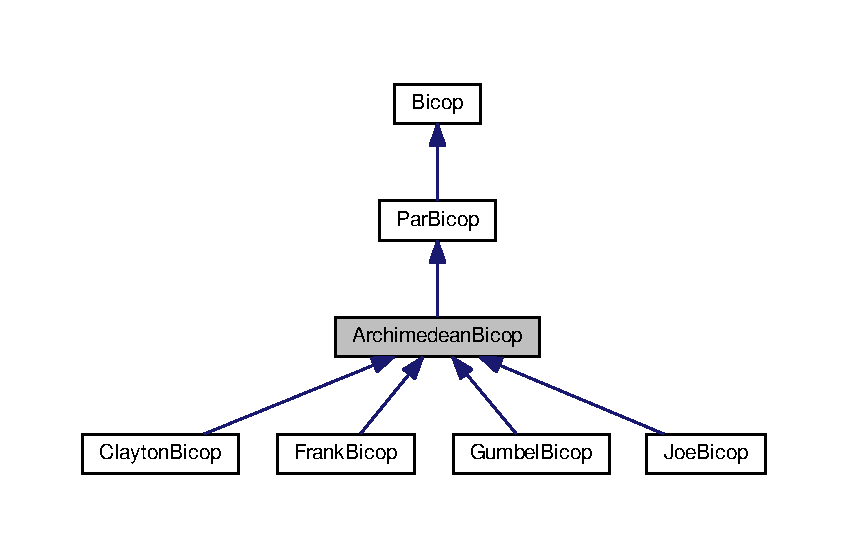
\includegraphics[width=350pt]{class_archimedean_bicop__inherit__graph}
\end{center}
\end{figure}


Collaboration diagram for Archimedean\+Bicop\+:\nopagebreak
\begin{figure}[H]
\begin{center}
\leavevmode
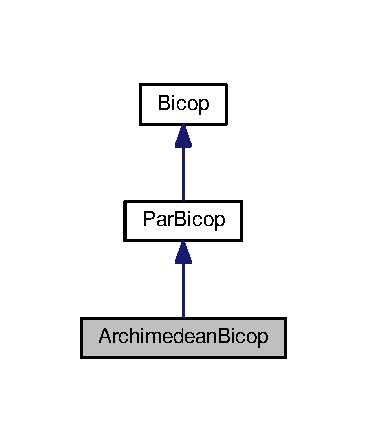
\includegraphics[width=178pt]{class_archimedean_bicop__coll__graph}
\end{center}
\end{figure}
\subsection*{Public Member Functions}
\begin{DoxyCompactItemize}
\item 
Vec\+Xd {\bfseries pdf\+\_\+default} (const Mat\+Xd \&u)\hypertarget{class_archimedean_bicop_adee082ce9b2f7cc4a3408d67ed6b49f5}{}\label{class_archimedean_bicop_adee082ce9b2f7cc4a3408d67ed6b49f5}

\item 
Vec\+Xd {\bfseries hfunc1\+\_\+default} (const Mat\+Xd \&u)\hypertarget{class_archimedean_bicop_a912effaac24a1c94aa1e1d4b08819d75}{}\label{class_archimedean_bicop_a912effaac24a1c94aa1e1d4b08819d75}

\item 
Vec\+Xd {\bfseries hfunc2\+\_\+default} (const Mat\+Xd \&u)\hypertarget{class_archimedean_bicop_a1651e16c4534ca99cd58eaf8602b8525}{}\label{class_archimedean_bicop_a1651e16c4534ca99cd58eaf8602b8525}

\item 
Vec\+Xd {\bfseries hinv1\+\_\+default} (const Mat\+Xd \&u)\hypertarget{class_archimedean_bicop_a5c5a8569bad4be9e92ccd4434305806b}{}\label{class_archimedean_bicop_a5c5a8569bad4be9e92ccd4434305806b}

\item 
Vec\+Xd {\bfseries hinv2\+\_\+default} (const Mat\+Xd \&u)\hypertarget{class_archimedean_bicop_a6bac4cee0e824719b107477a06caf19e}{}\label{class_archimedean_bicop_a6bac4cee0e824719b107477a06caf19e}

\item 
virtual Vec\+Xd {\bfseries generator} (const Vec\+Xd \&u)=0\hypertarget{class_archimedean_bicop_a9b79997308dc154a23808b84a863c563}{}\label{class_archimedean_bicop_a9b79997308dc154a23808b84a863c563}

\item 
virtual Vec\+Xd {\bfseries generator\+\_\+inv} (const Vec\+Xd \&u)=0\hypertarget{class_archimedean_bicop_af12082f1046554e0121b2c7d93148f13}{}\label{class_archimedean_bicop_af12082f1046554e0121b2c7d93148f13}

\item 
virtual Vec\+Xd {\bfseries generator\+\_\+derivative} (const Vec\+Xd \&u)=0\hypertarget{class_archimedean_bicop_a9a18bbc021eb033c5b7d992d6d572b9b}{}\label{class_archimedean_bicop_a9a18bbc021eb033c5b7d992d6d572b9b}

\item 
virtual Vec\+Xd {\bfseries generator\+\_\+derivative2} (const Vec\+Xd \&u)=0\hypertarget{class_archimedean_bicop_a16d7c2474e7e9bd16fa60a02550762ed}{}\label{class_archimedean_bicop_a16d7c2474e7e9bd16fa60a02550762ed}

\item 
void \hyperlink{class_archimedean_bicop_afc56334b1c34406b5148386d9b7e5f43}{flip} ()\hypertarget{class_archimedean_bicop_afc56334b1c34406b5148386d9b7e5f43}{}\label{class_archimedean_bicop_afc56334b1c34406b5148386d9b7e5f43}

\begin{DoxyCompactList}\small\item\em Adjust the copula to a flipping of arguments (u,v) -\/$>$ (v,u) \end{DoxyCompactList}\end{DoxyCompactItemize}
\subsection*{Additional Inherited Members}


The documentation for this class was generated from the following files\+:\begin{DoxyCompactItemize}
\item 
/home/n5/dev/cpp/vinecopulib/include/bicop\+\_\+archimedean.\+hpp\item 
/home/n5/dev/cpp/vinecopulib/src/bicop\+\_\+archimedean.\+cpp\end{DoxyCompactItemize}

\hypertarget{class_bb1_bicop}{}\section{Bb1\+Bicop Class Reference}
\label{class_bb1_bicop}\index{Bb1\+Bicop@{Bb1\+Bicop}}


Inheritance diagram for Bb1\+Bicop\+:\nopagebreak
\begin{figure}[H]
\begin{center}
\leavevmode
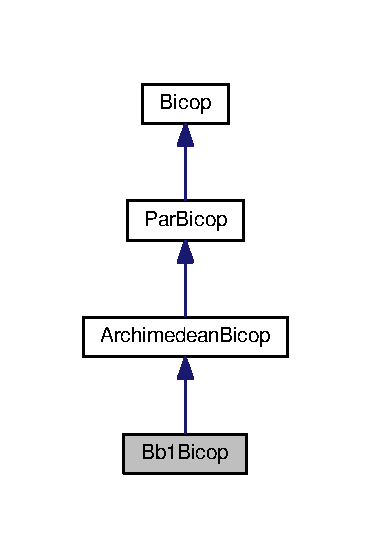
\includegraphics[width=178pt]{class_bb1_bicop__inherit__graph}
\end{center}
\end{figure}


Collaboration diagram for Bb1\+Bicop\+:\nopagebreak
\begin{figure}[H]
\begin{center}
\leavevmode
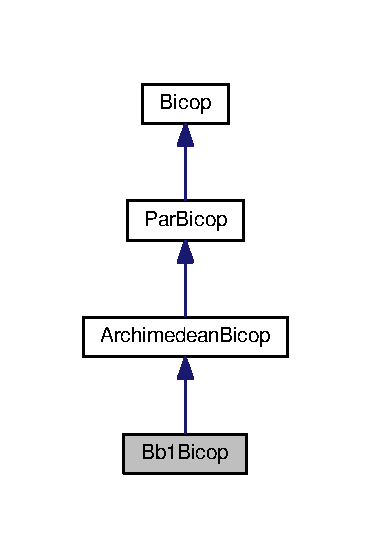
\includegraphics[width=178pt]{class_bb1_bicop__coll__graph}
\end{center}
\end{figure}
\subsection*{Public Member Functions}
\begin{DoxyCompactItemize}
\item 
{\bfseries Bb1\+Bicop} (const Vec\+Xd \&parameters)\hypertarget{class_bb1_bicop_a0c3efb2b45ece6695e75a5186e9b7d5b}{}\label{class_bb1_bicop_a0c3efb2b45ece6695e75a5186e9b7d5b}

\item 
{\bfseries Bb1\+Bicop} (const Vec\+Xd \&parameters, const int \&rotation)\hypertarget{class_bb1_bicop_af12e3c65691728cbc8304e26345c8974}{}\label{class_bb1_bicop_af12e3c65691728cbc8304e26345c8974}

\item 
Vec\+Xd {\bfseries generator} (const Vec\+Xd \&u)\hypertarget{class_bb1_bicop_ac87047a969a5ca3a6548d23d0c16711b}{}\label{class_bb1_bicop_ac87047a969a5ca3a6548d23d0c16711b}

\item 
Vec\+Xd {\bfseries generator\+\_\+inv} (const Vec\+Xd \&u)\hypertarget{class_bb1_bicop_aa6c69a5d19f28d6832505dd48d3fa4e8}{}\label{class_bb1_bicop_aa6c69a5d19f28d6832505dd48d3fa4e8}

\item 
Vec\+Xd {\bfseries generator\+\_\+derivative} (const Vec\+Xd \&u)\hypertarget{class_bb1_bicop_a7e1bd159b0412e74b4420ef802207c3e}{}\label{class_bb1_bicop_a7e1bd159b0412e74b4420ef802207c3e}

\item 
Vec\+Xd {\bfseries generator\+\_\+derivative2} (const Vec\+Xd \&u)\hypertarget{class_bb1_bicop_ad8d2b10bf538a4a95afff99d7897745f}{}\label{class_bb1_bicop_ad8d2b10bf538a4a95afff99d7897745f}

\item 
double {\bfseries parameters\+\_\+to\+\_\+tau} (const Vec\+Xd \&par)\hypertarget{class_bb1_bicop_af57fdfff6d26ef5cfc22e1ce02b23be7}{}\label{class_bb1_bicop_af57fdfff6d26ef5cfc22e1ce02b23be7}

\end{DoxyCompactItemize}
\subsection*{Additional Inherited Members}


The documentation for this class was generated from the following files\+:\begin{DoxyCompactItemize}
\item 
/home/n5/dev/cpp/vinecopulib/include/bicop\+\_\+bb1.\+hpp\item 
/home/n5/dev/cpp/vinecopulib/src/bicop\+\_\+bb1.\+cpp\end{DoxyCompactItemize}

\hypertarget{class_bb6_bicop}{}\section{Bb6\+Bicop Class Reference}
\label{class_bb6_bicop}\index{Bb6\+Bicop@{Bb6\+Bicop}}


Inheritance diagram for Bb6\+Bicop\+:\nopagebreak
\begin{figure}[H]
\begin{center}
\leavevmode
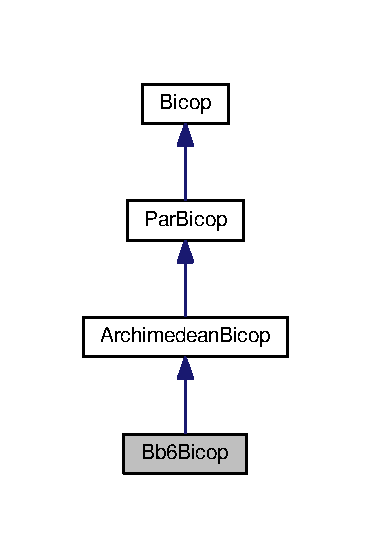
\includegraphics[width=178pt]{class_bb6_bicop__inherit__graph}
\end{center}
\end{figure}


Collaboration diagram for Bb6\+Bicop\+:\nopagebreak
\begin{figure}[H]
\begin{center}
\leavevmode
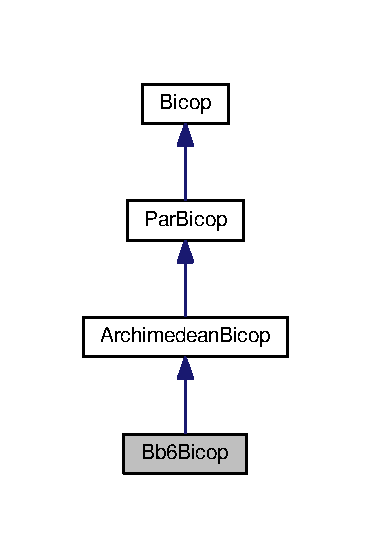
\includegraphics[width=178pt]{class_bb6_bicop__coll__graph}
\end{center}
\end{figure}
\subsection*{Public Member Functions}
\begin{DoxyCompactItemize}
\item 
{\bfseries Bb6\+Bicop} (const Vec\+Xd \&parameters)\hypertarget{class_bb6_bicop_afabf95772c3ecb4e999c2e5b00d8319c}{}\label{class_bb6_bicop_afabf95772c3ecb4e999c2e5b00d8319c}

\item 
{\bfseries Bb6\+Bicop} (const Vec\+Xd \&parameters, const int \&rotation)\hypertarget{class_bb6_bicop_a79525991f317ee6c20538f3b8e60780e}{}\label{class_bb6_bicop_a79525991f317ee6c20538f3b8e60780e}

\item 
Vec\+Xd {\bfseries generator} (const Vec\+Xd \&u)\hypertarget{class_bb6_bicop_a9bfb6b16340d34ff8e8eb626a059b78b}{}\label{class_bb6_bicop_a9bfb6b16340d34ff8e8eb626a059b78b}

\item 
Vec\+Xd {\bfseries generator\+\_\+inv} (const Vec\+Xd \&u)\hypertarget{class_bb6_bicop_ae381624eaadfa33e08eaa25eaf713590}{}\label{class_bb6_bicop_ae381624eaadfa33e08eaa25eaf713590}

\item 
Vec\+Xd {\bfseries generator\+\_\+derivative} (const Vec\+Xd \&u)\hypertarget{class_bb6_bicop_aa23265ee279e0cfba8af0594a1cac0e2}{}\label{class_bb6_bicop_aa23265ee279e0cfba8af0594a1cac0e2}

\item 
Vec\+Xd {\bfseries generator\+\_\+derivative2} (const Vec\+Xd \&u)\hypertarget{class_bb6_bicop_ae94d666bdbcf39d973148b7382893653}{}\label{class_bb6_bicop_ae94d666bdbcf39d973148b7382893653}

\item 
double {\bfseries parameters\+\_\+to\+\_\+tau} (const Vec\+Xd \&par)\hypertarget{class_bb6_bicop_ad12d84dddfb2a2aef8f8837a8df9570e}{}\label{class_bb6_bicop_ad12d84dddfb2a2aef8f8837a8df9570e}

\end{DoxyCompactItemize}
\subsection*{Additional Inherited Members}


The documentation for this class was generated from the following files\+:\begin{DoxyCompactItemize}
\item 
/home/n5/dev/cpp/vinecopulib/include/bicop\+\_\+bb6.\+hpp\item 
/home/n5/dev/cpp/vinecopulib/src/bicop\+\_\+bb6.\+cpp\end{DoxyCompactItemize}

\hypertarget{class_bb7_bicop}{}\section{Bb7\+Bicop Class Reference}
\label{class_bb7_bicop}\index{Bb7\+Bicop@{Bb7\+Bicop}}


Inheritance diagram for Bb7\+Bicop\+:\nopagebreak
\begin{figure}[H]
\begin{center}
\leavevmode
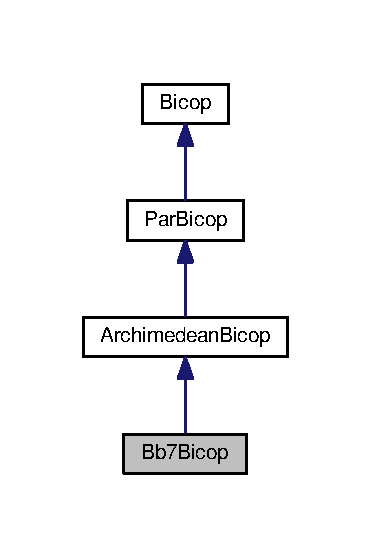
\includegraphics[width=178pt]{class_bb7_bicop__inherit__graph}
\end{center}
\end{figure}


Collaboration diagram for Bb7\+Bicop\+:\nopagebreak
\begin{figure}[H]
\begin{center}
\leavevmode
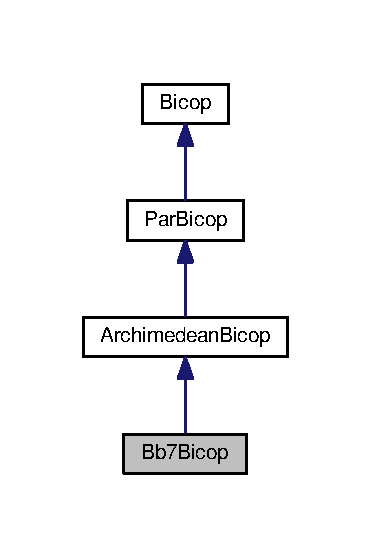
\includegraphics[width=178pt]{class_bb7_bicop__coll__graph}
\end{center}
\end{figure}
\subsection*{Public Member Functions}
\begin{DoxyCompactItemize}
\item 
{\bfseries Bb7\+Bicop} (const Vec\+Xd \&parameters)\hypertarget{class_bb7_bicop_afdab924db2ca1ce4e844079a8ece2c3c}{}\label{class_bb7_bicop_afdab924db2ca1ce4e844079a8ece2c3c}

\item 
{\bfseries Bb7\+Bicop} (const Vec\+Xd \&parameters, const int \&rotation)\hypertarget{class_bb7_bicop_a743d4bc3dc98acc793639b5b71e0dd50}{}\label{class_bb7_bicop_a743d4bc3dc98acc793639b5b71e0dd50}

\item 
Vec\+Xd {\bfseries generator} (const Vec\+Xd \&u)\hypertarget{class_bb7_bicop_a517cbe6415b9604e6be776d1a4960a14}{}\label{class_bb7_bicop_a517cbe6415b9604e6be776d1a4960a14}

\item 
Vec\+Xd {\bfseries generator\+\_\+inv} (const Vec\+Xd \&u)\hypertarget{class_bb7_bicop_a933701dad803f12849377c1e4f7cfefa}{}\label{class_bb7_bicop_a933701dad803f12849377c1e4f7cfefa}

\item 
Vec\+Xd {\bfseries generator\+\_\+derivative} (const Vec\+Xd \&u)\hypertarget{class_bb7_bicop_a37f336c2f58917f68a4c92ec117cf902}{}\label{class_bb7_bicop_a37f336c2f58917f68a4c92ec117cf902}

\item 
Vec\+Xd {\bfseries generator\+\_\+derivative2} (const Vec\+Xd \&u)\hypertarget{class_bb7_bicop_a6daf84cf601f12c066104fe9765d48b6}{}\label{class_bb7_bicop_a6daf84cf601f12c066104fe9765d48b6}

\item 
double {\bfseries parameters\+\_\+to\+\_\+tau} (const Vec\+Xd \&par)\hypertarget{class_bb7_bicop_abb052403535f812b716265d8ab347bdb}{}\label{class_bb7_bicop_abb052403535f812b716265d8ab347bdb}

\end{DoxyCompactItemize}
\subsection*{Additional Inherited Members}


The documentation for this class was generated from the following files\+:\begin{DoxyCompactItemize}
\item 
/home/n5/dev/cpp/vinecopulib/include/bicop\+\_\+bb7.\+hpp\item 
/home/n5/dev/cpp/vinecopulib/src/bicop\+\_\+bb7.\+cpp\end{DoxyCompactItemize}

\hypertarget{class_bb8_bicop}{}\section{Bb8\+Bicop Class Reference}
\label{class_bb8_bicop}\index{Bb8\+Bicop@{Bb8\+Bicop}}


Inheritance diagram for Bb8\+Bicop\+:\nopagebreak
\begin{figure}[H]
\begin{center}
\leavevmode
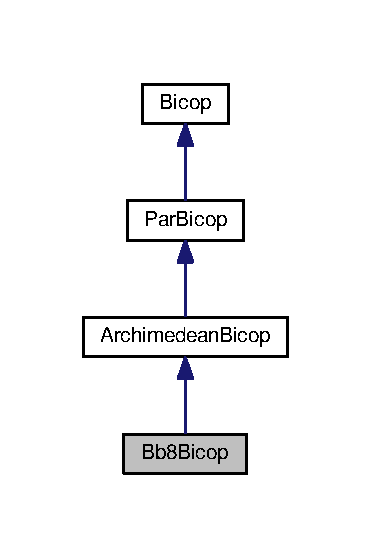
\includegraphics[width=178pt]{class_bb8_bicop__inherit__graph}
\end{center}
\end{figure}


Collaboration diagram for Bb8\+Bicop\+:\nopagebreak
\begin{figure}[H]
\begin{center}
\leavevmode
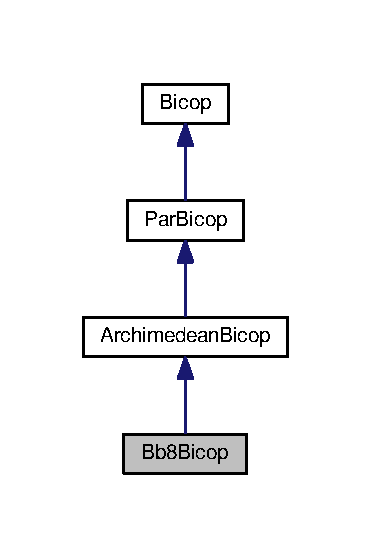
\includegraphics[width=178pt]{class_bb8_bicop__coll__graph}
\end{center}
\end{figure}
\subsection*{Public Member Functions}
\begin{DoxyCompactItemize}
\item 
{\bfseries Bb8\+Bicop} (const Vec\+Xd \&parameters)\hypertarget{class_bb8_bicop_a13fc1d0023c12f94ab3c012b32f4b9bc}{}\label{class_bb8_bicop_a13fc1d0023c12f94ab3c012b32f4b9bc}

\item 
{\bfseries Bb8\+Bicop} (const Vec\+Xd \&parameters, const int \&rotation)\hypertarget{class_bb8_bicop_a1a6942067c4bbfe44293d71538d8d5ef}{}\label{class_bb8_bicop_a1a6942067c4bbfe44293d71538d8d5ef}

\item 
Vec\+Xd {\bfseries generator} (const Vec\+Xd \&u)\hypertarget{class_bb8_bicop_a1c319afe3c9857a9ed58719a348d6a8d}{}\label{class_bb8_bicop_a1c319afe3c9857a9ed58719a348d6a8d}

\item 
Vec\+Xd {\bfseries generator\+\_\+inv} (const Vec\+Xd \&u)\hypertarget{class_bb8_bicop_a578ab4567cec20f6eca4fcf420584e3e}{}\label{class_bb8_bicop_a578ab4567cec20f6eca4fcf420584e3e}

\item 
Vec\+Xd {\bfseries generator\+\_\+derivative} (const Vec\+Xd \&u)\hypertarget{class_bb8_bicop_a2d5495d2f0a5482449e50ff02b652f4a}{}\label{class_bb8_bicop_a2d5495d2f0a5482449e50ff02b652f4a}

\item 
Vec\+Xd {\bfseries generator\+\_\+derivative2} (const Vec\+Xd \&u)\hypertarget{class_bb8_bicop_a6e9bfaad15aa46a537028570f20d7f54}{}\label{class_bb8_bicop_a6e9bfaad15aa46a537028570f20d7f54}

\item 
double {\bfseries parameters\+\_\+to\+\_\+tau} (const Vec\+Xd \&par)\hypertarget{class_bb8_bicop_ad6856da75e5003053858b40d6ab84a38}{}\label{class_bb8_bicop_ad6856da75e5003053858b40d6ab84a38}

\end{DoxyCompactItemize}
\subsection*{Additional Inherited Members}


The documentation for this class was generated from the following files\+:\begin{DoxyCompactItemize}
\item 
/home/n5/dev/cpp/vinecopulib/include/bicop\+\_\+bb8.\+hpp\item 
/home/n5/dev/cpp/vinecopulib/src/bicop\+\_\+bb8.\+cpp\end{DoxyCompactItemize}

\hypertarget{class_bicop}{}\section{Bicop Class Reference}
\label{class_bicop}\index{Bicop@{Bicop}}


{\ttfamily \#include $<$bicop\+\_\+class.\+hpp$>$}



Inheritance diagram for Bicop\+:\nopagebreak
\begin{figure}[H]
\begin{center}
\leavevmode
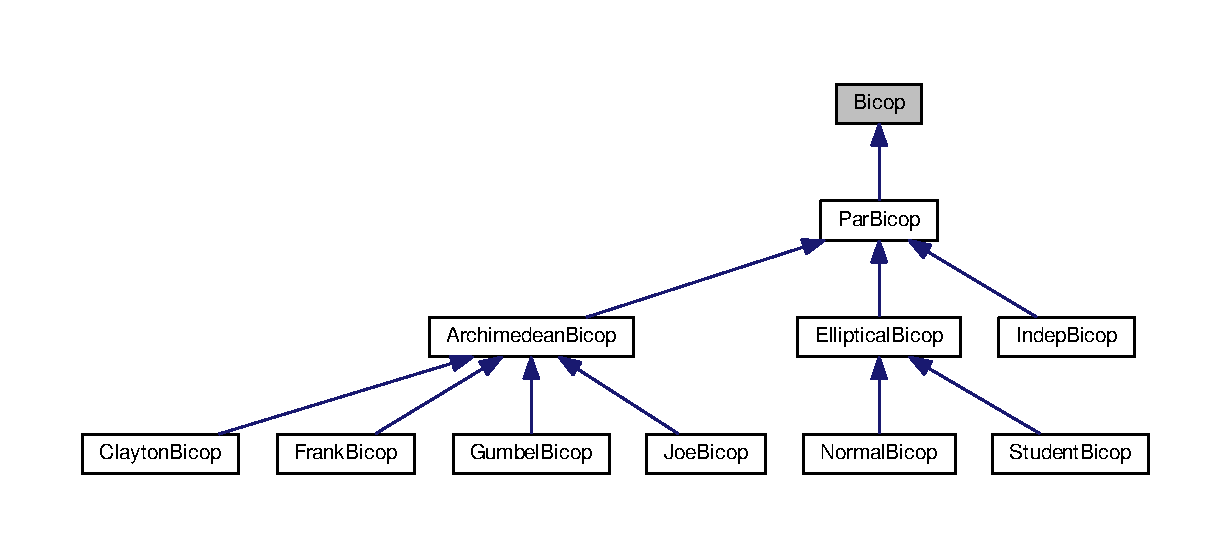
\includegraphics[width=350pt]{class_bicop__inherit__graph}
\end{center}
\end{figure}
\subsection*{Public Member Functions}
\begin{DoxyCompactItemize}
\item 
Vec\+Xd {\bfseries pdf} (const Mat\+Xd \&u)
\item 
Vec\+Xd {\bfseries hfunc1} (const Mat\+Xd \&u)
\item 
Vec\+Xd {\bfseries hfunc2} (const Mat\+Xd \&u)
\item 
Vec\+Xd {\bfseries hinv1} (const Mat\+Xd \&u)
\item 
Vec\+Xd {\bfseries hinv2} (const Mat\+Xd \&u)
\item 
Mat\+Xd \hyperlink{class_bicop_afa62d40a17e096cc0f7e769fb2a1285d}{simulate} (const int \&n)
\item 
virtual double \hyperlink{class_bicop_a21f37d9e51460c13be57e48c3d1e7ba4}{calculate\+\_\+npars} ()=0\hypertarget{class_bicop_a21f37d9e51460c13be57e48c3d1e7ba4}{}\label{class_bicop_a21f37d9e51460c13be57e48c3d1e7ba4}

\begin{DoxyCompactList}\small\item\em Get number of parameters. \end{DoxyCompactList}\item 
double \hyperlink{class_bicop_abe228ece449fb66996f91b0fcfed60d3}{calculate\+\_\+tau} ()\hypertarget{class_bicop_abe228ece449fb66996f91b0fcfed60d3}{}\label{class_bicop_abe228ece449fb66996f91b0fcfed60d3}

\begin{DoxyCompactList}\small\item\em Calculate the theoretical Kendall\textquotesingle{}s tau. \end{DoxyCompactList}\item 
virtual double {\bfseries parameters\+\_\+to\+\_\+tau} (const Vec\+Xd \&parameters)=0\hypertarget{class_bicop_aadd4f372b89a2389348893633ec238ba}{}\label{class_bicop_aadd4f372b89a2389348893633ec238ba}

\item 
Vec\+Xd \hyperlink{class_bicop_af20cc82a278f7c5a40dca399402caf10}{tau\+\_\+to\+\_\+parameters} (const double \&tau)\hypertarget{class_bicop_af20cc82a278f7c5a40dca399402caf10}{}\label{class_bicop_af20cc82a278f7c5a40dca399402caf10}

\begin{DoxyCompactList}\small\item\em Extract the copula parameter from Kendall\textquotesingle{}s tau whenever possible. \end{DoxyCompactList}\item 
virtual void \hyperlink{class_bicop_ac7d72dc620a2de66f6c1136329d1b4a3}{flip} ()=0\hypertarget{class_bicop_ac7d72dc620a2de66f6c1136329d1b4a3}{}\label{class_bicop_ac7d72dc620a2de66f6c1136329d1b4a3}

\begin{DoxyCompactList}\small\item\em Adjust the copula to a flipping of arguments (u,v) -\/$>$ (v,u) \end{DoxyCompactList}\end{DoxyCompactItemize}
{\bf }\par
\begin{DoxyCompactItemize}
\item 
virtual void \hyperlink{class_bicop_a0ff40d8054e11ed8aaa4956c7fd84e89}{fit} (const Mat\+Xd \&data, std\+::string method)=0
\item 
double {\bfseries loglik} (const Mat\+Xd \&u)\hypertarget{class_bicop_a994d28aa99b881425f012605aef3ae68}{}\label{class_bicop_a994d28aa99b881425f012605aef3ae68}

\item 
double {\bfseries aic} (const Mat\+Xd \&u)\hypertarget{class_bicop_adb4aecd877fc32cc857e2477d5bddf9b}{}\label{class_bicop_adb4aecd877fc32cc857e2477d5bddf9b}

\item 
double {\bfseries bic} (const Mat\+Xd \&u)\hypertarget{class_bicop_a68ee43f29c026aaf8157673c1ddf29b2}{}\label{class_bicop_a68ee43f29c026aaf8157673c1ddf29b2}

\end{DoxyCompactItemize}

{\bf }\par
\begin{DoxyCompactItemize}
\item 
int \hyperlink{class_bicop_a78a564f6e071e8dba7bcd93fdd1b05a4}{get\+\_\+family} () const 
\item 
int {\bfseries get\+\_\+rotation} () const \hypertarget{class_bicop_a0cf41f139c731d37841a411be5123155}{}\label{class_bicop_a0cf41f139c731d37841a411be5123155}

\item 
std\+::string {\bfseries get\+\_\+association\+\_\+direction} () const \hypertarget{class_bicop_a6758285bf2e354bbfbf8f8e0465567ba}{}\label{class_bicop_a6758285bf2e354bbfbf8f8e0465567ba}

\item 
Vec\+Xd {\bfseries get\+\_\+parameters} () const \hypertarget{class_bicop_a5ae1eb1665235ea822f0f62b69085047}{}\label{class_bicop_a5ae1eb1665235ea822f0f62b69085047}

\item 
Mat\+Xd {\bfseries get\+\_\+parameters\+\_\+bounds} () const \hypertarget{class_bicop_af3387cb6498e8b08c23d442a437ef6e0}{}\label{class_bicop_af3387cb6498e8b08c23d442a437ef6e0}

\item 
void {\bfseries set\+\_\+rotation} (const int \&rotation)\hypertarget{class_bicop_af5cded47298fa11fc0f997d7a873cf92}{}\label{class_bicop_af5cded47298fa11fc0f997d7a873cf92}

\item 
void {\bfseries set\+\_\+parameters} (const Vec\+Xd \&parameters)\hypertarget{class_bicop_a86d6d832e19d4e947fad68590e6f1b40}{}\label{class_bicop_a86d6d832e19d4e947fad68590e6f1b40}

\end{DoxyCompactItemize}

\subsection*{Static Public Member Functions}
\begin{DoxyCompactItemize}
\item 
static std\+::shared\+\_\+ptr$<$ \hyperlink{class_bicop}{Bicop} $>$ \hyperlink{class_bicop_acb60163725518f4ccfd7694272014686}{create} (const int \&family, const int \&rotation)
\item 
static std\+::shared\+\_\+ptr$<$ \hyperlink{class_bicop}{Bicop} $>$ \hyperlink{class_bicop_a4bfa38e69a96cc8a7c689e1161942e46}{create} (const int \&family, const Vec\+Xd \&parameters, const int \&rotation)
\item 
static std\+::shared\+\_\+ptr$<$ \hyperlink{class_bicop}{Bicop} $>$ \hyperlink{class_bicop_a6b1c154595bb17cd73f81cb4f563a776}{select} (const Mat\+Xd \&data, std\+::string selection\+\_\+criterion, std\+::vector$<$ int $>$ family\+\_\+set, bool use\+\_\+rotations, bool preselect\+\_\+families, std\+::string method)
\end{DoxyCompactItemize}
\subsection*{Protected Member Functions}
\begin{DoxyCompactItemize}
\item 
virtual Vec\+Xd {\bfseries pdf\+\_\+default} (const Mat\+Xd \&u)=0\hypertarget{class_bicop_a89e76fb74a9a4583cd74ce7bd72b5821}{}\label{class_bicop_a89e76fb74a9a4583cd74ce7bd72b5821}

\item 
virtual Vec\+Xd {\bfseries hfunc1\+\_\+default} (const Mat\+Xd \&u)=0\hypertarget{class_bicop_a60b997ec055f573034fc1736470ed7db}{}\label{class_bicop_a60b997ec055f573034fc1736470ed7db}

\item 
virtual Vec\+Xd {\bfseries hfunc2\+\_\+default} (const Mat\+Xd \&u)=0\hypertarget{class_bicop_afb7f326409f22b6b65e46f89dcf5ee1a}{}\label{class_bicop_afb7f326409f22b6b65e46f89dcf5ee1a}

\item 
virtual Vec\+Xd {\bfseries hinv1\+\_\+default} (const Mat\+Xd \&u)=0\hypertarget{class_bicop_a401bdcb4172c55b3d5f0c2a0db30ca43}{}\label{class_bicop_a401bdcb4172c55b3d5f0c2a0db30ca43}

\item 
virtual Vec\+Xd {\bfseries hinv2\+\_\+default} (const Mat\+Xd \&u)=0\hypertarget{class_bicop_a046b0fdc43eed27002f0b7c3bc9a9ddb}{}\label{class_bicop_a046b0fdc43eed27002f0b7c3bc9a9ddb}

\item 
Vec\+Xd \hyperlink{class_bicop_abd517becaa97834eac56b0d1a0c7a666}{hinv1\+\_\+num} (const Mat\+Xd \&u)
\item 
Vec\+Xd {\bfseries hinv2\+\_\+num} (const Mat\+Xd \&u)\hypertarget{class_bicop_a2b262e9e2adee0c215da47467f1dec45}{}\label{class_bicop_a2b262e9e2adee0c215da47467f1dec45}

\item 
Mat\+Xd \hyperlink{class_bicop_a48dc314b01b0c5b0adb307d27d4dd53e}{cut\+\_\+and\+\_\+rotate} (const Mat\+Xd \&u)
\item 
Mat\+Xd {\bfseries swap\+\_\+cols} (const Mat\+Xd \&u)\hypertarget{class_bicop_a96e06c8996e378d56d9e87ff4d1a24ac}{}\label{class_bicop_a96e06c8996e378d56d9e87ff4d1a24ac}

\end{DoxyCompactItemize}
\subsection*{Protected Attributes}
\begin{DoxyCompactItemize}
\item 
int {\bfseries family\+\_\+}\hypertarget{class_bicop_a3d546f9b8c6507002cae18b9fdcb4544}{}\label{class_bicop_a3d546f9b8c6507002cae18b9fdcb4544}

\item 
std\+::string {\bfseries family\+\_\+name\+\_\+}\hypertarget{class_bicop_ae87af8dcf838aa9342baf814f1a9c0c7}{}\label{class_bicop_ae87af8dcf838aa9342baf814f1a9c0c7}

\item 
int {\bfseries rotation\+\_\+}\hypertarget{class_bicop_a606833e2ea1d17a318dd20d67d01b40a}{}\label{class_bicop_a606833e2ea1d17a318dd20d67d01b40a}

\item 
std\+::string {\bfseries association\+\_\+direction\+\_\+}\hypertarget{class_bicop_a407914da267317da3f588632e4b95aa3}{}\label{class_bicop_a407914da267317da3f588632e4b95aa3}

\item 
Vec\+Xd {\bfseries parameters\+\_\+}\hypertarget{class_bicop_ade78fec591e6699a808b63104709b23a}{}\label{class_bicop_ade78fec591e6699a808b63104709b23a}

\item 
Mat\+Xd {\bfseries parameters\+\_\+bounds\+\_\+}\hypertarget{class_bicop_aa1253f11c251ea6d9f4020317e4346ab}{}\label{class_bicop_aa1253f11c251ea6d9f4020317e4346ab}

\end{DoxyCompactItemize}


\subsection{Detailed Description}
A class for bivariate copulas

The \hyperlink{class_bicop}{Bicop} class is abstract, you cannot create an instance of this class, but only of the derived classes. 

\subsection{Member Function Documentation}
\index{Bicop@{Bicop}!create@{create}}
\index{create@{create}!Bicop@{Bicop}}
\subsubsection[{\texorpdfstring{create(const int \&family, const int \&rotation)}{create(const int &family, const int &rotation)}}]{\setlength{\rightskip}{0pt plus 5cm}Bicop\+Ptr Bicop\+::create (
\begin{DoxyParamCaption}
\item[{const int \&}]{family, }
\item[{const int \&}]{rotation}
\end{DoxyParamCaption}
)\hspace{0.3cm}{\ttfamily [static]}}\hypertarget{class_bicop_acb60163725518f4ccfd7694272014686}{}\label{class_bicop_acb60163725518f4ccfd7694272014686}
Create a bivariate copula using the default contructor


\begin{DoxyParams}{Parameters}
{\em family} & the copula family. \\
\hline
{\em rotation} & the rotation type. \\
\hline
\end{DoxyParams}
\begin{DoxyReturn}{Returns}
A pointer to an object that inherits from {\ttfamily \hyperlink{class_bicop}{Bicop}}. 
\end{DoxyReturn}
\index{Bicop@{Bicop}!create@{create}}
\index{create@{create}!Bicop@{Bicop}}
\subsubsection[{\texorpdfstring{create(const int \&family, const Vec\+Xd \&parameters, const int \&rotation)}{create(const int &family, const VecXd &parameters, const int &rotation)}}]{\setlength{\rightskip}{0pt plus 5cm}Bicop\+Ptr Bicop\+::create (
\begin{DoxyParamCaption}
\item[{const int \&}]{family, }
\item[{const Vec\+Xd \&}]{parameters, }
\item[{const int \&}]{rotation}
\end{DoxyParamCaption}
)\hspace{0.3cm}{\ttfamily [static]}}\hypertarget{class_bicop_a4bfa38e69a96cc8a7c689e1161942e46}{}\label{class_bicop_a4bfa38e69a96cc8a7c689e1161942e46}
Create a bivariate copula with a specified parameters vector


\begin{DoxyParams}{Parameters}
{\em family} & the copula family. \\
\hline
{\em par} & the copula parameters (must be compatible with family). \\
\hline
{\em rotation} & the rotation type. \\
\hline
\end{DoxyParams}
\begin{DoxyReturn}{Returns}
A pointer to an object that inherits from {\ttfamily \hyperlink{class_bicop}{Bicop}}. 
\end{DoxyReturn}
\index{Bicop@{Bicop}!cut\+\_\+and\+\_\+rotate@{cut\+\_\+and\+\_\+rotate}}
\index{cut\+\_\+and\+\_\+rotate@{cut\+\_\+and\+\_\+rotate}!Bicop@{Bicop}}
\subsubsection[{\texorpdfstring{cut\+\_\+and\+\_\+rotate(const Mat\+Xd \&u)}{cut_and_rotate(const MatXd &u)}}]{\setlength{\rightskip}{0pt plus 5cm}Mat\+Xd Bicop\+::cut\+\_\+and\+\_\+rotate (
\begin{DoxyParamCaption}
\item[{const Mat\+Xd \&}]{u}
\end{DoxyParamCaption}
)\hspace{0.3cm}{\ttfamily [protected]}}\hypertarget{class_bicop_a48dc314b01b0c5b0adb307d27d4dd53e}{}\label{class_bicop_a48dc314b01b0c5b0adb307d27d4dd53e}
Data manipulations for rotated families


\begin{DoxyParams}{Parameters}
{\em u} & $m \times 2$ matrix of evaluation points. \\
\hline
\end{DoxyParams}
\index{Bicop@{Bicop}!fit@{fit}}
\index{fit@{fit}!Bicop@{Bicop}}
\subsubsection[{\texorpdfstring{fit(const Mat\+Xd \&data, std\+::string method)=0}{fit(const MatXd &data, std::string method)=0}}]{\setlength{\rightskip}{0pt plus 5cm}virtual void Bicop\+::fit (
\begin{DoxyParamCaption}
\item[{const Mat\+Xd \&}]{data, }
\item[{std\+::string}]{method}
\end{DoxyParamCaption}
)\hspace{0.3cm}{\ttfamily [pure virtual]}}\hypertarget{class_bicop_a0ff40d8054e11ed8aaa4956c7fd84e89}{}\label{class_bicop_a0ff40d8054e11ed8aaa4956c7fd84e89}
fitstats Fit methods and statistics


\begin{DoxyParams}{Parameters}
{\em u} & $m \times 2$ matrix of observations. \\
\hline
\end{DoxyParams}


Implemented in \hyperlink{class_par_bicop_aeab5e7031792bebc04a401a8f135d3a0}{Par\+Bicop}, and \hyperlink{class_trafokernel_bicop_ae5da9284cd058b02878614059d8ce078}{Trafokernel\+Bicop}.

\index{Bicop@{Bicop}!get\+\_\+family@{get\+\_\+family}}
\index{get\+\_\+family@{get\+\_\+family}!Bicop@{Bicop}}
\subsubsection[{\texorpdfstring{get\+\_\+family() const }{get_family() const }}]{\setlength{\rightskip}{0pt plus 5cm}int Bicop\+::get\+\_\+family (
\begin{DoxyParamCaption}
{}
\end{DoxyParamCaption}
) const\hspace{0.3cm}{\ttfamily [inline]}}\hypertarget{class_bicop_a78a564f6e071e8dba7bcd93fdd1b05a4}{}\label{class_bicop_a78a564f6e071e8dba7bcd93fdd1b05a4}
Getters and setters. \index{Bicop@{Bicop}!hinv1\+\_\+num@{hinv1\+\_\+num}}
\index{hinv1\+\_\+num@{hinv1\+\_\+num}!Bicop@{Bicop}}
\subsubsection[{\texorpdfstring{hinv1\+\_\+num(const Mat\+Xd \&u)}{hinv1_num(const MatXd &u)}}]{\setlength{\rightskip}{0pt plus 5cm}Vec\+Xd Bicop\+::hinv1\+\_\+num (
\begin{DoxyParamCaption}
\item[{const Mat\+Xd \&}]{u}
\end{DoxyParamCaption}
)\hspace{0.3cm}{\ttfamily [protected]}}\hypertarget{class_bicop_abd517becaa97834eac56b0d1a0c7a666}{}\label{class_bicop_abd517becaa97834eac56b0d1a0c7a666}
Numerical inversion of h-\/functions

These are generic functions to invert the hfunctions numerically. They can be used in derived classes to define {\ttfamily hinv1} and {\ttfamily hinv2}.


\begin{DoxyParams}{Parameters}
{\em u} & $m \times 2$ matrix of evaluation points. \\
\hline
\end{DoxyParams}
\index{Bicop@{Bicop}!select@{select}}
\index{select@{select}!Bicop@{Bicop}}
\subsubsection[{\texorpdfstring{select(const Mat\+Xd \&data, std\+::string selection\+\_\+criterion, std\+::vector$<$ int $>$ family\+\_\+set, bool use\+\_\+rotations, bool preselect\+\_\+families, std\+::string method)}{select(const MatXd &data, std::string selection_criterion, std::vector< int > family_set, bool use_rotations, bool preselect_families, std::string method)}}]{\setlength{\rightskip}{0pt plus 5cm}Bicop\+Ptr Bicop\+::select (
\begin{DoxyParamCaption}
\item[{const Mat\+Xd \&}]{data, }
\item[{std\+::string}]{selection\+\_\+criterion, }
\item[{std\+::vector$<$ int $>$}]{family\+\_\+set, }
\item[{bool}]{use\+\_\+rotations, }
\item[{bool}]{preselect\+\_\+families, }
\item[{std\+::string}]{method}
\end{DoxyParamCaption}
)\hspace{0.3cm}{\ttfamily [static]}}\hypertarget{class_bicop_a6b1c154595bb17cd73f81cb4f563a776}{}\label{class_bicop_a6b1c154595bb17cd73f81cb4f563a776}
Select a bivariate copula


\begin{DoxyParams}{Parameters}
{\em data} & the data to fit the bivariate copula. \\
\hline
{\em selection\+\_\+criterion} & the selection criterion (\char`\"{}aic\char`\"{} or \char`\"{}bic\char`\"{}). \\
\hline
{\em family\+\_\+set} & the set of copula families to consider (if empty, then all families are included). \\
\hline
{\em use\+\_\+rotations} & whether rotations in the familyset are included. \\
\hline
{\em preselect\+\_\+families} & whether to exclude families before fitting based on symmetry properties of the data. \\
\hline
{\em method} & indicates the estimation method\+: either maximum likelihood estimation (method = \char`\"{}mle\char`\"{}) or inversion of Kendall\textquotesingle{}s tau (method = \char`\"{}itau\char`\"{}). When method = \char`\"{}itau\char`\"{} is used with families having more than one parameter, the main dependence parameter is found by inverting the Kendall\textquotesingle{}s tau and the remainders by a profile likelihood optimization. \\
\hline
\end{DoxyParams}
\begin{DoxyReturn}{Returns}
A pointer to an object that inherits from {\ttfamily \hyperlink{class_bicop}{Bicop}}. 
\end{DoxyReturn}
\index{Bicop@{Bicop}!simulate@{simulate}}
\index{simulate@{simulate}!Bicop@{Bicop}}
\subsubsection[{\texorpdfstring{simulate(const int \&n)}{simulate(const int &n)}}]{\setlength{\rightskip}{0pt plus 5cm}Mat\+Xd Bicop\+::simulate (
\begin{DoxyParamCaption}
\item[{const int \&}]{n}
\end{DoxyParamCaption}
)}\hypertarget{class_bicop_afa62d40a17e096cc0f7e769fb2a1285d}{}\label{class_bicop_afa62d40a17e096cc0f7e769fb2a1285d}
Simulate from a bivariate copula


\begin{DoxyParams}{Parameters}
{\em n} & number of observations. \\
\hline
\end{DoxyParams}


The documentation for this class was generated from the following files\+:\begin{DoxyCompactItemize}
\item 
/home/n5/dev/cpp/vinecopulib/include/bicop\+\_\+class.\+hpp\item 
/home/n5/dev/cpp/vinecopulib/src/bicop\+\_\+class.\+cpp\end{DoxyCompactItemize}

\hypertarget{class_clayton_bicop}{}\section{Clayton\+Bicop Class Reference}
\label{class_clayton_bicop}\index{Clayton\+Bicop@{Clayton\+Bicop}}


Inheritance diagram for Clayton\+Bicop\+:\nopagebreak
\begin{figure}[H]
\begin{center}
\leavevmode
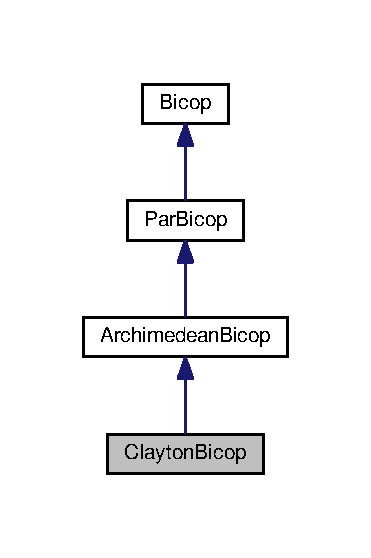
\includegraphics[width=178pt]{class_clayton_bicop__inherit__graph}
\end{center}
\end{figure}


Collaboration diagram for Clayton\+Bicop\+:\nopagebreak
\begin{figure}[H]
\begin{center}
\leavevmode
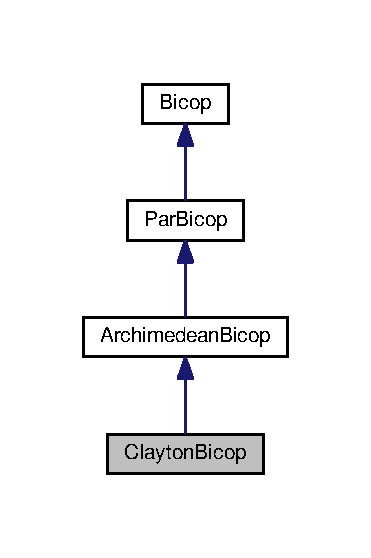
\includegraphics[width=178pt]{class_clayton_bicop__coll__graph}
\end{center}
\end{figure}
\subsection*{Public Member Functions}
\begin{DoxyCompactItemize}
\item 
{\bfseries Clayton\+Bicop} (const Vec\+Xd \&parameters)\hypertarget{class_clayton_bicop_a40ae835970aa67c3aacea800a831cc52}{}\label{class_clayton_bicop_a40ae835970aa67c3aacea800a831cc52}

\item 
{\bfseries Clayton\+Bicop} (const Vec\+Xd \&parameters, const int \&rotation)\hypertarget{class_clayton_bicop_a7b28e2ac34943f2b69616efffedcf720}{}\label{class_clayton_bicop_a7b28e2ac34943f2b69616efffedcf720}

\item 
Vec\+Xd {\bfseries generator} (const Vec\+Xd \&u)\hypertarget{class_clayton_bicop_a9763aabca37806261b8ecd6c46f4cf95}{}\label{class_clayton_bicop_a9763aabca37806261b8ecd6c46f4cf95}

\item 
Vec\+Xd {\bfseries generator\+\_\+inv} (const Vec\+Xd \&u)\hypertarget{class_clayton_bicop_a295caa6493575640a96201414dbf398f}{}\label{class_clayton_bicop_a295caa6493575640a96201414dbf398f}

\item 
Vec\+Xd {\bfseries generator\+\_\+derivative} (const Vec\+Xd \&u)\hypertarget{class_clayton_bicop_ab009f6aa6036ad92d83a3d185e6234d8}{}\label{class_clayton_bicop_ab009f6aa6036ad92d83a3d185e6234d8}

\item 
Vec\+Xd {\bfseries generator\+\_\+derivative2} (const Vec\+Xd \&u)\hypertarget{class_clayton_bicop_af24c631fbf12bcf3f52724fcf926cfef}{}\label{class_clayton_bicop_af24c631fbf12bcf3f52724fcf926cfef}

\item 
Vec\+Xd {\bfseries hinv1\+\_\+default} (const Mat\+Xd \&u)\hypertarget{class_clayton_bicop_a54ee65a9403fab88aa713f50c57971b7}{}\label{class_clayton_bicop_a54ee65a9403fab88aa713f50c57971b7}

\item 
Vec\+Xd {\bfseries tau\+\_\+to\+\_\+parameters} (const double \&tau)\hypertarget{class_clayton_bicop_a7ffb38cb5802a8d4d45f401ac5aab83b}{}\label{class_clayton_bicop_a7ffb38cb5802a8d4d45f401ac5aab83b}

\item 
double {\bfseries parameters\+\_\+to\+\_\+tau} (const Vec\+Xd \&parameters)\hypertarget{class_clayton_bicop_a5eba5ab351ad17df7d633c7c96f6cbdf}{}\label{class_clayton_bicop_a5eba5ab351ad17df7d633c7c96f6cbdf}

\end{DoxyCompactItemize}
\subsection*{Additional Inherited Members}


The documentation for this class was generated from the following files\+:\begin{DoxyCompactItemize}
\item 
/home/n5/dev/cpp/vinecopulib/include/bicop\+\_\+clayton.\+hpp\item 
/home/n5/dev/cpp/vinecopulib/src/bicop\+\_\+clayton.\+cpp\end{DoxyCompactItemize}

\hypertarget{structstructselect__tools_1_1_edge_properties}{}\section{structselect\+\_\+tools\+:\+:Edge\+Properties Struct Reference}
\label{structstructselect__tools_1_1_edge_properties}\index{structselect\+\_\+tools\+::\+Edge\+Properties@{structselect\+\_\+tools\+::\+Edge\+Properties}}
\subsection*{Public Attributes}
\begin{DoxyCompactItemize}
\item 
std\+::vector$<$ int $>$ {\bfseries conditioning}\hypertarget{structstructselect__tools_1_1_edge_properties_a9f1c09d462b487e2cb45bbe6fa2f6368}{}\label{structstructselect__tools_1_1_edge_properties_a9f1c09d462b487e2cb45bbe6fa2f6368}

\item 
std\+::vector$<$ int $>$ {\bfseries conditioned}\hypertarget{structstructselect__tools_1_1_edge_properties_a1b0d50e8466ddc845c726a50ae16ebea}{}\label{structstructselect__tools_1_1_edge_properties_a1b0d50e8466ddc845c726a50ae16ebea}

\item 
std\+::vector$<$ int $>$ {\bfseries all\+\_\+indices}\hypertarget{structstructselect__tools_1_1_edge_properties_a702ffe89a46787f06659890db25a0611}{}\label{structstructselect__tools_1_1_edge_properties_a702ffe89a46787f06659890db25a0611}

\item 
Mat\+Xd {\bfseries pc\+\_\+data}\hypertarget{structstructselect__tools_1_1_edge_properties_a65df14de91b2be8d9a1492791e6b65bc}{}\label{structstructselect__tools_1_1_edge_properties_a65df14de91b2be8d9a1492791e6b65bc}

\item 
Vec\+Xd {\bfseries hfunc1}\hypertarget{structstructselect__tools_1_1_edge_properties_adc800b6e2bb72a0a68b4675a7daeda96}{}\label{structstructselect__tools_1_1_edge_properties_adc800b6e2bb72a0a68b4675a7daeda96}

\item 
Vec\+Xd {\bfseries hfunc2}\hypertarget{structstructselect__tools_1_1_edge_properties_a951d87593c49216772be6f5a6f7baf9c}{}\label{structstructselect__tools_1_1_edge_properties_a951d87593c49216772be6f5a6f7baf9c}

\item 
double {\bfseries empirical\+\_\+tau}\hypertarget{structstructselect__tools_1_1_edge_properties_a24eb86105437d0a61b63dbe26d08d579}{}\label{structstructselect__tools_1_1_edge_properties_a24eb86105437d0a61b63dbe26d08d579}

\item 
Bicop\+Ptr {\bfseries pair\+\_\+copula}\hypertarget{structstructselect__tools_1_1_edge_properties_a6bfce8ceccc789baad98184646a40c17}{}\label{structstructselect__tools_1_1_edge_properties_a6bfce8ceccc789baad98184646a40c17}

\end{DoxyCompactItemize}


The documentation for this struct was generated from the following file\+:\begin{DoxyCompactItemize}
\item 
/home/n5/dev/cpp/vinecopulib/include/structselect\+\_\+tools.\+hpp\end{DoxyCompactItemize}

\hypertarget{class_elliptical_bicop}{\section{Elliptical\+Bicop Class Reference}
\label{class_elliptical_bicop}\index{Elliptical\+Bicop@{Elliptical\+Bicop}}
}


Inheritance diagram for Elliptical\+Bicop\+:\nopagebreak
\begin{figure}[H]
\begin{center}
\leavevmode
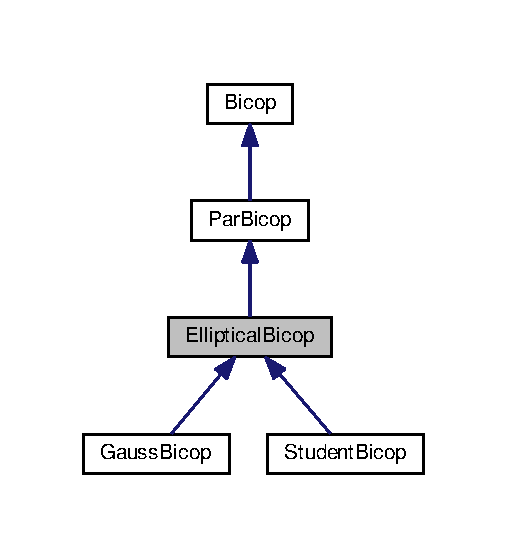
\includegraphics[width=243pt]{class_elliptical_bicop__inherit__graph}
\end{center}
\end{figure}


Collaboration diagram for Elliptical\+Bicop\+:\nopagebreak
\begin{figure}[H]
\begin{center}
\leavevmode
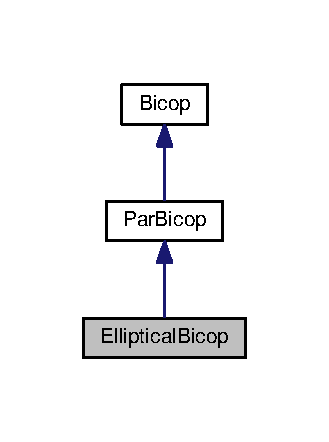
\includegraphics[width=158pt]{class_elliptical_bicop__coll__graph}
\end{center}
\end{figure}
\subsection*{Public Member Functions}
\begin{DoxyCompactItemize}
\item 
\hypertarget{class_elliptical_bicop_a9d859278685c80465d09dc8fe05b7d3d}{virtual Vec\+Xd {\bfseries pdf\+\_\+default} (const Mat\+Xd \&u)=0}\label{class_elliptical_bicop_a9d859278685c80465d09dc8fe05b7d3d}

\item 
\hypertarget{class_elliptical_bicop_ae4e47a0b9373b0f103b28fbacdaa58b8}{virtual Vec\+Xd {\bfseries hfunc1\+\_\+default} (const Mat\+Xd \&u)=0}\label{class_elliptical_bicop_ae4e47a0b9373b0f103b28fbacdaa58b8}

\item 
\hypertarget{class_elliptical_bicop_a18f5fa85bd6ed14d56e0b269c091ac3b}{Vec\+Xd {\bfseries hfunc2\+\_\+default} (const Mat\+Xd \&u)}\label{class_elliptical_bicop_a18f5fa85bd6ed14d56e0b269c091ac3b}

\item 
\hypertarget{class_elliptical_bicop_aa2a3700bc5dd43aade311985f96077e0}{virtual Vec\+Xd {\bfseries hinv1\+\_\+default} (const Mat\+Xd \&u)=0}\label{class_elliptical_bicop_aa2a3700bc5dd43aade311985f96077e0}

\item 
\hypertarget{class_elliptical_bicop_ac94477889cbd73c30eb7010001e9fec8}{Vec\+Xd {\bfseries hinv2\+\_\+default} (const Mat\+Xd \&u)}\label{class_elliptical_bicop_ac94477889cbd73c30eb7010001e9fec8}

\item 
\hypertarget{class_elliptical_bicop_a4a478ff32dddf4561c8d97041b943e1f}{Vec\+Xd {\bfseries tau\+\_\+to\+\_\+parameters} (const double \&tau)}\label{class_elliptical_bicop_a4a478ff32dddf4561c8d97041b943e1f}

\item 
\hypertarget{class_elliptical_bicop_a45f034c75af02d9b20b4af5c16754e5a}{double {\bfseries parameters\+\_\+to\+\_\+tau} (const Vec\+Xd \&parameters)}\label{class_elliptical_bicop_a45f034c75af02d9b20b4af5c16754e5a}

\item 
\hypertarget{class_elliptical_bicop_a176f55b005e74efe21abd01651ea8967}{void \hyperlink{class_elliptical_bicop_a176f55b005e74efe21abd01651ea8967}{flip} ()}\label{class_elliptical_bicop_a176f55b005e74efe21abd01651ea8967}

\begin{DoxyCompactList}\small\item\em Adjust the copula to a flipping of arguments (u,v) -\/$>$ (v,u) \end{DoxyCompactList}\end{DoxyCompactItemize}
\subsection*{Additional Inherited Members}

\hypertarget{class_frank_bicop}{}\section{Frank\+Bicop Class Reference}
\label{class_frank_bicop}\index{Frank\+Bicop@{Frank\+Bicop}}


Inheritance diagram for Frank\+Bicop\+:\nopagebreak
\begin{figure}[H]
\begin{center}
\leavevmode
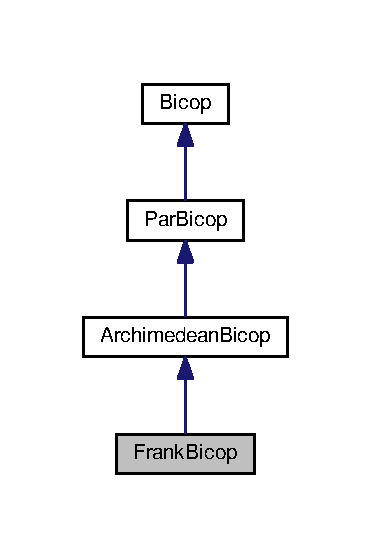
\includegraphics[width=178pt]{class_frank_bicop__inherit__graph}
\end{center}
\end{figure}


Collaboration diagram for Frank\+Bicop\+:\nopagebreak
\begin{figure}[H]
\begin{center}
\leavevmode
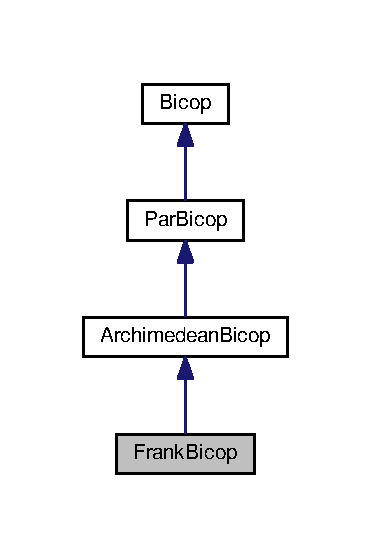
\includegraphics[width=178pt]{class_frank_bicop__coll__graph}
\end{center}
\end{figure}
\subsection*{Public Member Functions}
\begin{DoxyCompactItemize}
\item 
{\bfseries Frank\+Bicop} (const Vec\+Xd \&parameters)\hypertarget{class_frank_bicop_ae019221e15eba598f29d9120ac6d1f5c}{}\label{class_frank_bicop_ae019221e15eba598f29d9120ac6d1f5c}

\item 
{\bfseries Frank\+Bicop} (const Vec\+Xd \&parameters, const int \&rotation)\hypertarget{class_frank_bicop_af789907cefc0049b2ce6ea4596195d48}{}\label{class_frank_bicop_af789907cefc0049b2ce6ea4596195d48}

\item 
Vec\+Xd {\bfseries generator} (const Vec\+Xd \&u)\hypertarget{class_frank_bicop_aac20b71ec67ea5067c5342c085a0e306}{}\label{class_frank_bicop_aac20b71ec67ea5067c5342c085a0e306}

\item 
Vec\+Xd {\bfseries generator\+\_\+inv} (const Vec\+Xd \&u)\hypertarget{class_frank_bicop_a3e433ca2c858e95c11896d2d6a445648}{}\label{class_frank_bicop_a3e433ca2c858e95c11896d2d6a445648}

\item 
Vec\+Xd {\bfseries generator\+\_\+derivative} (const Vec\+Xd \&u)\hypertarget{class_frank_bicop_a19d2a80d449caa48d75690be81c2db02}{}\label{class_frank_bicop_a19d2a80d449caa48d75690be81c2db02}

\item 
Vec\+Xd {\bfseries generator\+\_\+derivative2} (const Vec\+Xd \&u)\hypertarget{class_frank_bicop_a07d9488138a598fa9aa770da2153f269}{}\label{class_frank_bicop_a07d9488138a598fa9aa770da2153f269}

\item 
Vec\+Xd {\bfseries tau\+\_\+to\+\_\+parameters} (const double \&tau)\hypertarget{class_frank_bicop_ad4c350e726aa9ca7682d77c3e4e6ed3c}{}\label{class_frank_bicop_ad4c350e726aa9ca7682d77c3e4e6ed3c}

\item 
double {\bfseries parameters\+\_\+to\+\_\+tau} (const Vec\+Xd \&par)\hypertarget{class_frank_bicop_a59f4a4bbe5eb724d18091c2cd379e268}{}\label{class_frank_bicop_a59f4a4bbe5eb724d18091c2cd379e268}

\end{DoxyCompactItemize}
\subsection*{Additional Inherited Members}


The documentation for this class was generated from the following files\+:\begin{DoxyCompactItemize}
\item 
/home/n5/dev/cpp/vinecopulib/include/bicop\+\_\+frank.\+hpp\item 
/home/n5/dev/cpp/vinecopulib/src/bicop\+\_\+frank.\+cpp\end{DoxyCompactItemize}

\hypertarget{class_gauss_bicop}{}\section{Gauss\+Bicop Class Reference}
\label{class_gauss_bicop}\index{Gauss\+Bicop@{Gauss\+Bicop}}


Inheritance diagram for Gauss\+Bicop\+:\nopagebreak
\begin{figure}[H]
\begin{center}
\leavevmode
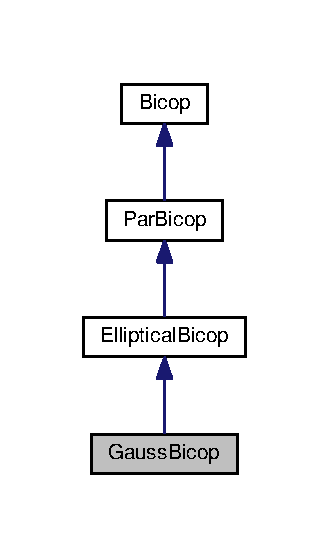
\includegraphics[width=158pt]{class_gauss_bicop__inherit__graph}
\end{center}
\end{figure}


Collaboration diagram for Gauss\+Bicop\+:\nopagebreak
\begin{figure}[H]
\begin{center}
\leavevmode
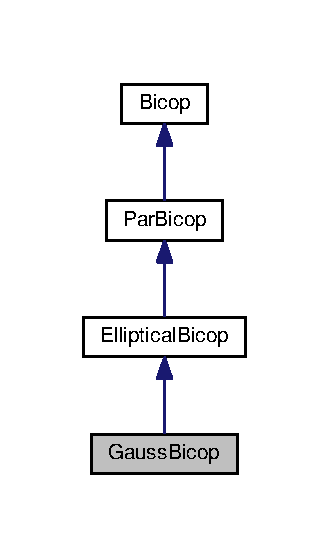
\includegraphics[width=158pt]{class_gauss_bicop__coll__graph}
\end{center}
\end{figure}
\subsection*{Public Member Functions}
\begin{DoxyCompactItemize}
\item 
{\bfseries Gauss\+Bicop} (const Vec\+Xd \&parameters)\hypertarget{class_gauss_bicop_a7701b11601e7d9cb0c49aa449440924e}{}\label{class_gauss_bicop_a7701b11601e7d9cb0c49aa449440924e}

\item 
{\bfseries Gauss\+Bicop} (const Vec\+Xd \&parameters, const int \&rotation)\hypertarget{class_gauss_bicop_aa3ca70729cc7f4b027dc660cf47bf908}{}\label{class_gauss_bicop_aa3ca70729cc7f4b027dc660cf47bf908}

\item 
Vec\+Xd {\bfseries pdf\+\_\+default} (const Mat\+Xd \&u)\hypertarget{class_gauss_bicop_ae12c6e56243c6f2d2878fa403f2ccb91}{}\label{class_gauss_bicop_ae12c6e56243c6f2d2878fa403f2ccb91}

\item 
Vec\+Xd {\bfseries hfunc1\+\_\+default} (const Mat\+Xd \&u)\hypertarget{class_gauss_bicop_a9a6e04b749c34920cc8c981dd8114c2b}{}\label{class_gauss_bicop_a9a6e04b749c34920cc8c981dd8114c2b}

\item 
Vec\+Xd {\bfseries hinv1\+\_\+default} (const Mat\+Xd \&u)\hypertarget{class_gauss_bicop_a298263b90ef2ab40190d4fe00bd9196c}{}\label{class_gauss_bicop_a298263b90ef2ab40190d4fe00bd9196c}

\end{DoxyCompactItemize}
\subsection*{Additional Inherited Members}


The documentation for this class was generated from the following files\+:\begin{DoxyCompactItemize}
\item 
/home/n5/dev/cpp/vinecopulib/include/bicop\+\_\+gauss.\+hpp\item 
/home/n5/dev/cpp/vinecopulib/src/bicop\+\_\+gauss.\+cpp\end{DoxyCompactItemize}

\hypertarget{class_gumbel_bicop}{}\section{Gumbel\+Bicop Class Reference}
\label{class_gumbel_bicop}\index{Gumbel\+Bicop@{Gumbel\+Bicop}}


Inheritance diagram for Gumbel\+Bicop\+:\nopagebreak
\begin{figure}[H]
\begin{center}
\leavevmode
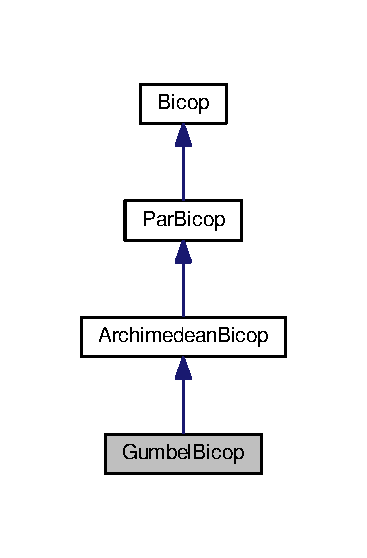
\includegraphics[width=178pt]{class_gumbel_bicop__inherit__graph}
\end{center}
\end{figure}


Collaboration diagram for Gumbel\+Bicop\+:\nopagebreak
\begin{figure}[H]
\begin{center}
\leavevmode
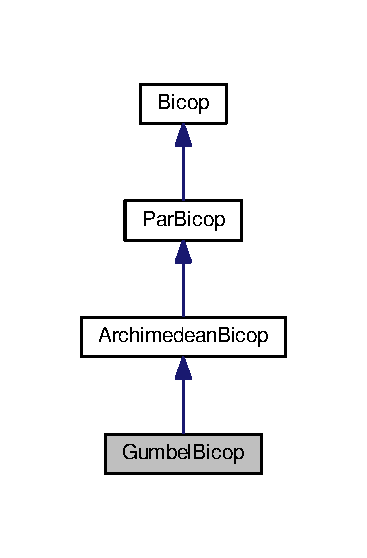
\includegraphics[width=178pt]{class_gumbel_bicop__coll__graph}
\end{center}
\end{figure}
\subsection*{Public Member Functions}
\begin{DoxyCompactItemize}
\item 
{\bfseries Gumbel\+Bicop} (const Vec\+Xd \&parameters)\hypertarget{class_gumbel_bicop_a96f6d7548161eefbc68999d52095eef3}{}\label{class_gumbel_bicop_a96f6d7548161eefbc68999d52095eef3}

\item 
{\bfseries Gumbel\+Bicop} (const Vec\+Xd \&parameters, const int \&rotation)\hypertarget{class_gumbel_bicop_a54f07cbf2630e03ddb81cbb1a07bbe9f}{}\label{class_gumbel_bicop_a54f07cbf2630e03ddb81cbb1a07bbe9f}

\item 
Vec\+Xd {\bfseries generator} (const Vec\+Xd \&u)\hypertarget{class_gumbel_bicop_a7462d2e917ed8f9c7c768bc763062000}{}\label{class_gumbel_bicop_a7462d2e917ed8f9c7c768bc763062000}

\item 
Vec\+Xd {\bfseries generator\+\_\+inv} (const Vec\+Xd \&u)\hypertarget{class_gumbel_bicop_a1aac5fc1926ebb1a7a5477fea8eafc4e}{}\label{class_gumbel_bicop_a1aac5fc1926ebb1a7a5477fea8eafc4e}

\item 
Vec\+Xd {\bfseries generator\+\_\+derivative} (const Vec\+Xd \&u)\hypertarget{class_gumbel_bicop_a04ad137cdb969fdcb38141dd55cc08ca}{}\label{class_gumbel_bicop_a04ad137cdb969fdcb38141dd55cc08ca}

\item 
Vec\+Xd {\bfseries generator\+\_\+derivative2} (const Vec\+Xd \&u)\hypertarget{class_gumbel_bicop_ab86b728ad0f0db50711e25defc39a1ad}{}\label{class_gumbel_bicop_ab86b728ad0f0db50711e25defc39a1ad}

\item 
Vec\+Xd {\bfseries hinv1\+\_\+default} (const Mat\+Xd \&u)\hypertarget{class_gumbel_bicop_ace2f375b5d67a02f3af9488ebe4120e5}{}\label{class_gumbel_bicop_ace2f375b5d67a02f3af9488ebe4120e5}

\item 
Vec\+Xd {\bfseries tau\+\_\+to\+\_\+parameters} (const double \&tau)\hypertarget{class_gumbel_bicop_a0128ce09c2184f9b71f4b54c2790ed84}{}\label{class_gumbel_bicop_a0128ce09c2184f9b71f4b54c2790ed84}

\item 
double {\bfseries parameters\+\_\+to\+\_\+tau} (const Vec\+Xd \&parameters)\hypertarget{class_gumbel_bicop_a6755267e48f12c29d943416c60e9f33f}{}\label{class_gumbel_bicop_a6755267e48f12c29d943416c60e9f33f}

\end{DoxyCompactItemize}
\subsection*{Additional Inherited Members}


The documentation for this class was generated from the following files\+:\begin{DoxyCompactItemize}
\item 
/home/n5/dev/cpp/vinecopulib/include/bicop\+\_\+gumbel.\+hpp\item 
/home/n5/dev/cpp/vinecopulib/src/bicop\+\_\+gumbel.\+cpp\end{DoxyCompactItemize}

\hypertarget{class_indep_bicop}{\section{Indep\+Bicop Class Reference}
\label{class_indep_bicop}\index{Indep\+Bicop@{Indep\+Bicop}}
}


Inheritance diagram for Indep\+Bicop\+:\nopagebreak
\begin{figure}[H]
\begin{center}
\leavevmode
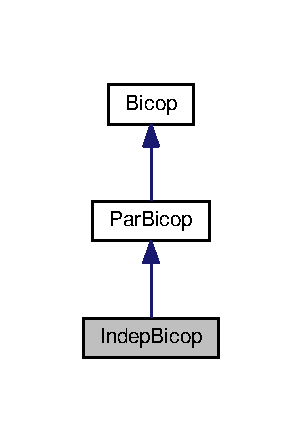
\includegraphics[width=144pt]{class_indep_bicop__inherit__graph}
\end{center}
\end{figure}


Collaboration diagram for Indep\+Bicop\+:\nopagebreak
\begin{figure}[H]
\begin{center}
\leavevmode
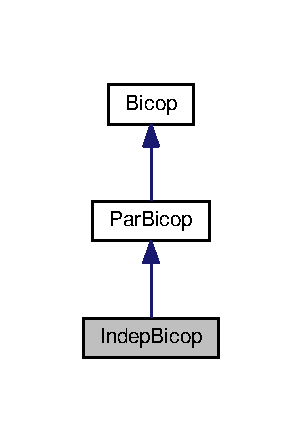
\includegraphics[width=144pt]{class_indep_bicop__coll__graph}
\end{center}
\end{figure}
\subsection*{Public Member Functions}
\begin{DoxyCompactItemize}
\item 
\hypertarget{class_indep_bicop_ab9f48d3291ac99c34e33c2f29b133e5d}{{\bfseries Indep\+Bicop} (const Vec\+Xd \&parameters)}\label{class_indep_bicop_ab9f48d3291ac99c34e33c2f29b133e5d}

\item 
\hypertarget{class_indep_bicop_ad7ead44250e4f421ec491b2d2a7eb030}{{\bfseries Indep\+Bicop} (const Vec\+Xd \&parameters, const int \&rotation)}\label{class_indep_bicop_ad7ead44250e4f421ec491b2d2a7eb030}

\item 
\hypertarget{class_indep_bicop_a533aeb27876d38d9836929a71b9bb223}{Vec\+Xd {\bfseries pdf\+\_\+default} (const Mat\+Xd \&u)}\label{class_indep_bicop_a533aeb27876d38d9836929a71b9bb223}

\item 
\hypertarget{class_indep_bicop_abac716dd22bc020d073d50dfc552c00e}{Vec\+Xd {\bfseries hfunc1\+\_\+default} (const Mat\+Xd \&u)}\label{class_indep_bicop_abac716dd22bc020d073d50dfc552c00e}

\item 
\hypertarget{class_indep_bicop_ae054353b15c15d68a02b36a804e54dfa}{Vec\+Xd {\bfseries hfunc2\+\_\+default} (const Mat\+Xd \&u)}\label{class_indep_bicop_ae054353b15c15d68a02b36a804e54dfa}

\item 
\hypertarget{class_indep_bicop_a61e64923f5b5a142d093c5b706893b93}{Vec\+Xd {\bfseries hinv1\+\_\+default} (const Mat\+Xd \&u)}\label{class_indep_bicop_a61e64923f5b5a142d093c5b706893b93}

\item 
\hypertarget{class_indep_bicop_a426311d78e6142d6f57e5a09080f9239}{Vec\+Xd {\bfseries hinv2\+\_\+default} (const Mat\+Xd \&u)}\label{class_indep_bicop_a426311d78e6142d6f57e5a09080f9239}

\item 
\hypertarget{class_indep_bicop_ae2bcd4c9c3fadb947cce3d1915ca6f57}{Vec\+Xd {\bfseries tau\+\_\+to\+\_\+parameters} (const double \&)}\label{class_indep_bicop_ae2bcd4c9c3fadb947cce3d1915ca6f57}

\item 
\hypertarget{class_indep_bicop_a1f9a8f4bf6d0fc6a053ded53eb35015a}{double {\bfseries parameters\+\_\+to\+\_\+tau} (const Vec\+Xd \&)}\label{class_indep_bicop_a1f9a8f4bf6d0fc6a053ded53eb35015a}

\item 
\hypertarget{class_indep_bicop_ab6e5a7670b984d685241b6c998ff3381}{void \hyperlink{class_indep_bicop_ab6e5a7670b984d685241b6c998ff3381}{flip} ()}\label{class_indep_bicop_ab6e5a7670b984d685241b6c998ff3381}

\begin{DoxyCompactList}\small\item\em Adjust the copula to a flipping of arguments (u,v) -\/$>$ (v,u) \end{DoxyCompactList}\end{DoxyCompactItemize}
\subsection*{Additional Inherited Members}

\hypertarget{class_interpolation_grid}{\section{Interpolation\+Grid Class Reference}
\label{class_interpolation_grid}\index{Interpolation\+Grid@{Interpolation\+Grid}}
}


{\ttfamily \#include $<$interpolation\+\_\+grid.\+hpp$>$}

\subsection*{Public Member Functions}
\begin{DoxyCompactItemize}
\item 
\hyperlink{class_interpolation_grid_aed2639844689b97483d665feb5d0d0f7}{Interpolation\+Grid} (const Vec\+Xd \&grid\+\_\+points, const Mat\+Xd \&values)
\item 
\hypertarget{class_interpolation_grid_a07cca3a1e214f98fc9bafa2a6379f789}{void {\bfseries flip} ()}\label{class_interpolation_grid_a07cca3a1e214f98fc9bafa2a6379f789}

\item 
Vec\+Xd \hyperlink{class_interpolation_grid_a9e65596940b5e561ef6332d2559feb57}{interpolate} (const Mat\+Xd \&x)
\item 
Vec\+Xd \hyperlink{class_interpolation_grid_a90af7bd3f2646109be939fc48b2284ca}{intergrate\+\_\+1d} (const Mat\+Xd \&u, const int \&cond\+\_\+var)
\item 
Vec\+Xd \hyperlink{class_interpolation_grid_aba233f98f869c2aeff0d920a1dd477d6}{inv\+\_\+intergrate\+\_\+1d} (const Mat\+Xd \&u, const int \&cond\+\_\+var)
\end{DoxyCompactItemize}


\subsection{Detailed Description}
A class for cubic spline interpolation of bivariate copulas

The class is used for implementing kernel estimators. It makes storing the observations obsolete and allows for fast numerical integration. 

\subsection{Constructor \& Destructor Documentation}
\hypertarget{class_interpolation_grid_aed2639844689b97483d665feb5d0d0f7}{\index{Interpolation\+Grid@{Interpolation\+Grid}!Interpolation\+Grid@{Interpolation\+Grid}}
\index{Interpolation\+Grid@{Interpolation\+Grid}!Interpolation\+Grid@{Interpolation\+Grid}}
\subsubsection[{Interpolation\+Grid}]{\setlength{\rightskip}{0pt plus 5cm}Interpolation\+Grid\+::\+Interpolation\+Grid (
\begin{DoxyParamCaption}
\item[{const Vec\+Xd \&}]{grid\+\_\+points, }
\item[{const Mat\+Xd \&}]{values}
\end{DoxyParamCaption}
)}}\label{class_interpolation_grid_aed2639844689b97483d665feb5d0d0f7}
Constructor


\begin{DoxyParams}{Parameters}
{\em grid\+\_\+points} & an ascending sequence of grid\+\_\+points; used in both dimensions. \\
\hline
{\em values} & a dxd matrix of copula density values evaluated at (grid\+\_\+points\+\_\+i, grid\+\_\+points\+\_\+j). \\
\hline
\end{DoxyParams}


\subsection{Member Function Documentation}
\hypertarget{class_interpolation_grid_a90af7bd3f2646109be939fc48b2284ca}{\index{Interpolation\+Grid@{Interpolation\+Grid}!intergrate\+\_\+1d@{intergrate\+\_\+1d}}
\index{intergrate\+\_\+1d@{intergrate\+\_\+1d}!Interpolation\+Grid@{Interpolation\+Grid}}
\subsubsection[{intergrate\+\_\+1d}]{\setlength{\rightskip}{0pt plus 5cm}Vec\+Xd Interpolation\+Grid\+::intergrate\+\_\+1d (
\begin{DoxyParamCaption}
\item[{const Mat\+Xd \&}]{u, }
\item[{const int \&}]{cond\+\_\+var}
\end{DoxyParamCaption}
)}}\label{class_interpolation_grid_a90af7bd3f2646109be939fc48b2284ca}
Integrate the grid along one axis


\begin{DoxyParams}{Parameters}
{\em u} & mx2 matrix of evaluation points \\
\hline
{\em cond\+\_\+var} & either 1 or 2; the axis considered fixed. \\
\hline
\end{DoxyParams}
\hypertarget{class_interpolation_grid_a9e65596940b5e561ef6332d2559feb57}{\index{Interpolation\+Grid@{Interpolation\+Grid}!interpolate@{interpolate}}
\index{interpolate@{interpolate}!Interpolation\+Grid@{Interpolation\+Grid}}
\subsubsection[{interpolate}]{\setlength{\rightskip}{0pt plus 5cm}Vec\+Xd Interpolation\+Grid\+::interpolate (
\begin{DoxyParamCaption}
\item[{const Mat\+Xd \&}]{x}
\end{DoxyParamCaption}
)}}\label{class_interpolation_grid_a9e65596940b5e561ef6332d2559feb57}
Interpolation in two dimensions


\begin{DoxyParams}{Parameters}
{\em x} & mx2 matrix of evaluation points. \\
\hline
\end{DoxyParams}
\hypertarget{class_interpolation_grid_aba233f98f869c2aeff0d920a1dd477d6}{\index{Interpolation\+Grid@{Interpolation\+Grid}!inv\+\_\+intergrate\+\_\+1d@{inv\+\_\+intergrate\+\_\+1d}}
\index{inv\+\_\+intergrate\+\_\+1d@{inv\+\_\+intergrate\+\_\+1d}!Interpolation\+Grid@{Interpolation\+Grid}}
\subsubsection[{inv\+\_\+intergrate\+\_\+1d}]{\setlength{\rightskip}{0pt plus 5cm}Vec\+Xd Interpolation\+Grid\+::inv\+\_\+intergrate\+\_\+1d (
\begin{DoxyParamCaption}
\item[{const Mat\+Xd \&}]{u, }
\item[{const int \&}]{cond\+\_\+var}
\end{DoxyParamCaption}
)}}\label{class_interpolation_grid_aba233f98f869c2aeff0d920a1dd477d6}
Inverse of integral along one axis of the grid


\begin{DoxyParams}{Parameters}
{\em u} & mx2 matrix of evaluation points \\
\hline
{\em cond\+\_\+var} & either 1 or 2; the axis considered fixed. \\
\hline
\end{DoxyParams}

\hypertarget{class_joe_bicop}{\section{Joe\+Bicop Class Reference}
\label{class_joe_bicop}\index{Joe\+Bicop@{Joe\+Bicop}}
}


Inheritance diagram for Joe\+Bicop\+:
\nopagebreak
\begin{figure}[H]
\begin{center}
\leavevmode
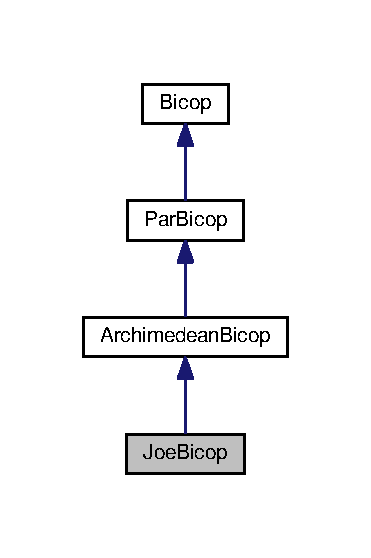
\includegraphics[width=176pt]{class_joe_bicop__inherit__graph}
\end{center}
\end{figure}


Collaboration diagram for Joe\+Bicop\+:
\nopagebreak
\begin{figure}[H]
\begin{center}
\leavevmode
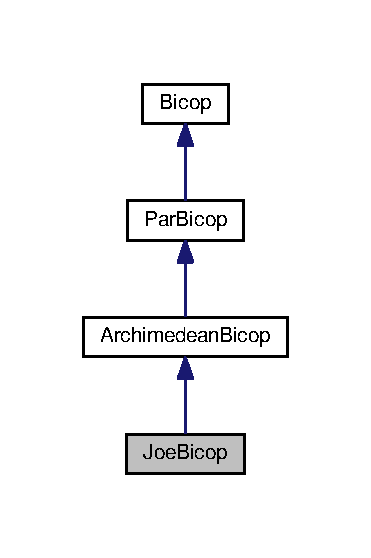
\includegraphics[width=176pt]{class_joe_bicop__coll__graph}
\end{center}
\end{figure}
\subsection*{Public Member Functions}
\begin{DoxyCompactItemize}
\item 
\hypertarget{class_joe_bicop_a8ddf492ef634fd120f8cce963f32014a}{{\bfseries Joe\+Bicop} (double theta)}\label{class_joe_bicop_a8ddf492ef634fd120f8cce963f32014a}

\item 
\hypertarget{class_joe_bicop_aab8dd1d752753480a930b6fa82ed0f4b}{{\bfseries Joe\+Bicop} (double theta, int rotation)}\label{class_joe_bicop_aab8dd1d752753480a930b6fa82ed0f4b}

\item 
\hypertarget{class_joe_bicop_a3a9cd4684de97041f271ce1f40c32fa2}{Vec\+Xd {\bfseries generator} (const Vec\+Xd \&u)}\label{class_joe_bicop_a3a9cd4684de97041f271ce1f40c32fa2}

\item 
\hypertarget{class_joe_bicop_ad4d4ff3ee52eac61b526f10a8b12c400}{Vec\+Xd {\bfseries generator\+\_\+inv} (const Vec\+Xd \&u)}\label{class_joe_bicop_ad4d4ff3ee52eac61b526f10a8b12c400}

\item 
\hypertarget{class_joe_bicop_a9ee3b11b81ae825369fc1a82f922d480}{Vec\+Xd {\bfseries generator\+\_\+derivative} (const Vec\+Xd \&u)}\label{class_joe_bicop_a9ee3b11b81ae825369fc1a82f922d480}

\item 
\hypertarget{class_joe_bicop_a7613e4c3cd33efac94cf2d1ee7b9869d}{Vec\+Xd {\bfseries generator\+\_\+derivative2} (const Vec\+Xd \&u)}\label{class_joe_bicop_a7613e4c3cd33efac94cf2d1ee7b9869d}

\item 
\hypertarget{class_joe_bicop_a40102f50e0cd111ad75a46acdfbd80ac}{Vec\+Xd {\bfseries hinv} (const Mat\+Xd \&u)}\label{class_joe_bicop_a40102f50e0cd111ad75a46acdfbd80ac}

\item 
\hypertarget{class_joe_bicop_a3e0bd20eb4e01bf762a24fa73ca0ce52}{double {\bfseries tau\+\_\+to\+\_\+par} (double \&tau)}\label{class_joe_bicop_a3e0bd20eb4e01bf762a24fa73ca0ce52}

\item 
\hypertarget{class_joe_bicop_aac2914100c2a16efe169b392f328673c}{double {\bfseries par\+\_\+to\+\_\+tau} (double \&par)}\label{class_joe_bicop_aac2914100c2a16efe169b392f328673c}

\item 
\hypertarget{class_joe_bicop_adf082c40e8205a0602ae676df684e0a1}{Mat\+Xd {\bfseries get\+\_\+bounds\+\_\+standard} ()}\label{class_joe_bicop_adf082c40e8205a0602ae676df684e0a1}

\end{DoxyCompactItemize}
\subsection*{Additional Inherited Members}


The documentation for this class was generated from the following files\+:\begin{DoxyCompactItemize}
\item 
/home/data/uni/\+Promotion/\+Cpp/vinecoplib/src/common/include/bicop\+\_\+joe.\+hpp\item 
/home/data/uni/\+Promotion/\+Cpp/vinecoplib/src/common/bicop\+\_\+joe.\+cpp\end{DoxyCompactItemize}

\hypertarget{class_kernel_bicop}{\section{Kernel\+Bicop Class Reference}
\label{class_kernel_bicop}\index{Kernel\+Bicop@{Kernel\+Bicop}}
}


Inheritance diagram for Kernel\+Bicop\+:\nopagebreak
\begin{figure}[H]
\begin{center}
\leavevmode
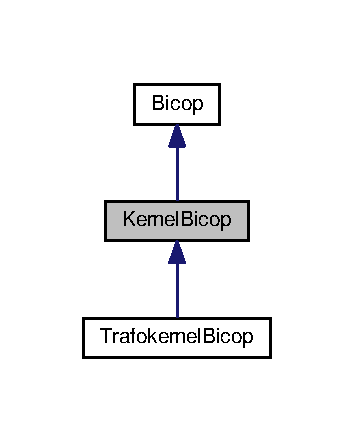
\includegraphics[width=170pt]{class_kernel_bicop__inherit__graph}
\end{center}
\end{figure}


Collaboration diagram for Kernel\+Bicop\+:\nopagebreak
\begin{figure}[H]
\begin{center}
\leavevmode
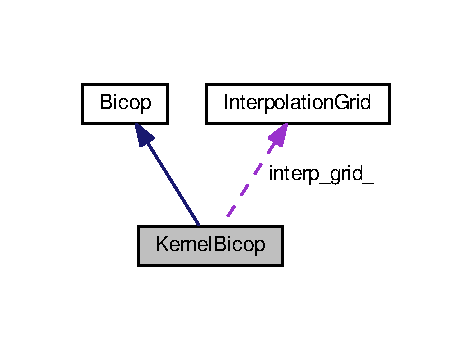
\includegraphics[width=226pt]{class_kernel_bicop__coll__graph}
\end{center}
\end{figure}
\subsection*{Public Member Functions}
\begin{DoxyCompactItemize}
\item 
\hypertarget{class_kernel_bicop_aa5c384abe680e15e68ee753ba07383b9}{Vec\+Xd {\bfseries pdf\+\_\+default} (const Mat\+Xd \&u)}\label{class_kernel_bicop_aa5c384abe680e15e68ee753ba07383b9}

\item 
\hypertarget{class_kernel_bicop_a813b02c149cdfdecd19f7d75b48a5750}{Vec\+Xd {\bfseries hfunc1\+\_\+default} (const Mat\+Xd \&u)}\label{class_kernel_bicop_a813b02c149cdfdecd19f7d75b48a5750}

\item 
\hypertarget{class_kernel_bicop_a50d6ee40f8ad1cacf26207aeca593ce7}{Vec\+Xd {\bfseries hfunc2\+\_\+default} (const Mat\+Xd \&u)}\label{class_kernel_bicop_a50d6ee40f8ad1cacf26207aeca593ce7}

\item 
\hypertarget{class_kernel_bicop_aef4490ec07370b9d94da42ffc66472bb}{Vec\+Xd {\bfseries hinv1\+\_\+default} (const Mat\+Xd \&u)}\label{class_kernel_bicop_aef4490ec07370b9d94da42ffc66472bb}

\item 
\hypertarget{class_kernel_bicop_aaa8f2330ce0be70f2963ad2c9fbe3bc9}{Vec\+Xd {\bfseries hinv2\+\_\+default} (const Mat\+Xd \&u)}\label{class_kernel_bicop_aaa8f2330ce0be70f2963ad2c9fbe3bc9}

\item 
\hypertarget{class_kernel_bicop_a75af40b7db1c24278ea373f0633a9b22}{double {\bfseries parameters\+\_\+to\+\_\+tau} (const Vec\+Xd \&)}\label{class_kernel_bicop_a75af40b7db1c24278ea373f0633a9b22}

\item 
\hypertarget{class_kernel_bicop_a631fd1cf2a05f30353ed9048839fae85}{double \hyperlink{class_kernel_bicop_a631fd1cf2a05f30353ed9048839fae85}{calculate\+\_\+npars} ()}\label{class_kernel_bicop_a631fd1cf2a05f30353ed9048839fae85}

\begin{DoxyCompactList}\small\item\em Get number of parameters. \end{DoxyCompactList}\item 
\hypertarget{class_kernel_bicop_a671e7f0f6d43e4eed35aceda3f70ab58}{void \hyperlink{class_kernel_bicop_a671e7f0f6d43e4eed35aceda3f70ab58}{flip} ()}\label{class_kernel_bicop_a671e7f0f6d43e4eed35aceda3f70ab58}

\begin{DoxyCompactList}\small\item\em Adjust the copula to a flipping of arguments (u,v) -\/$>$ (v,u) \end{DoxyCompactList}\end{DoxyCompactItemize}
\subsection*{Protected Attributes}
\begin{DoxyCompactItemize}
\item 
\hypertarget{class_kernel_bicop_a38c072985270dd91e2424d4453ee94a0}{\hyperlink{class_interpolation_grid}{Interpolation\+Grid} {\bfseries interp\+\_\+grid\+\_\+}}\label{class_kernel_bicop_a38c072985270dd91e2424d4453ee94a0}

\item 
\hypertarget{class_kernel_bicop_aab4f58d0b48ffba37fc617ba7ea9de56}{double {\bfseries npars\+\_\+}}\label{class_kernel_bicop_aab4f58d0b48ffba37fc617ba7ea9de56}

\end{DoxyCompactItemize}
\subsection*{Additional Inherited Members}

\hypertarget{classoptimization__tools_1_1_n_lopt_controls}{}\section{optimization\+\_\+tools\+:\+:N\+Lopt\+Controls Class Reference}
\label{classoptimization__tools_1_1_n_lopt_controls}\index{optimization\+\_\+tools\+::\+N\+Lopt\+Controls@{optimization\+\_\+tools\+::\+N\+Lopt\+Controls}}


{\ttfamily \#include $<$optimization\+\_\+tools.\+hpp$>$}

\subsection*{Public Member Functions}
\begin{DoxyCompactItemize}
\item 
\hyperlink{classoptimization__tools_1_1_n_lopt_controls_a79c68f622a830310faab4b7053404537}{N\+Lopt\+Controls} ()
\item 
\hyperlink{classoptimization__tools_1_1_n_lopt_controls_a32a9c83dccfd6465bbe2781461754b53}{N\+Lopt\+Controls} (double xtol\+\_\+rel, double xtol\+\_\+abs, double ftol\+\_\+rel, double ftol\+\_\+abs, int maxeval)
\item 
void \hyperlink{classoptimization__tools_1_1_n_lopt_controls_abadc98747c00b03d2ca1438a90e0f7ea}{set\+\_\+controls} (nlopt\+::opt $\ast$opt)
\end{DoxyCompactItemize}
{\bf }\par
\begin{DoxyCompactItemize}
\item 
double \hyperlink{classoptimization__tools_1_1_n_lopt_controls_a3b9ab6936b1058c3e54b06740ef3ea98}{get\+\_\+xtol\+\_\+rel} ()
\item 
double {\bfseries get\+\_\+xtol\+\_\+abs} ()\hypertarget{classoptimization__tools_1_1_n_lopt_controls_a499c5dc12d817d4bfbf9e0299d3ee59d}{}\label{classoptimization__tools_1_1_n_lopt_controls_a499c5dc12d817d4bfbf9e0299d3ee59d}

\item 
double {\bfseries get\+\_\+ftol\+\_\+rel} ()\hypertarget{classoptimization__tools_1_1_n_lopt_controls_ad969617f00cfc10828de474d8280ac2b}{}\label{classoptimization__tools_1_1_n_lopt_controls_ad969617f00cfc10828de474d8280ac2b}

\item 
double {\bfseries get\+\_\+ftol\+\_\+abs} ()\hypertarget{classoptimization__tools_1_1_n_lopt_controls_ab6a7f0d0199b9c66a79fa35f19acee04}{}\label{classoptimization__tools_1_1_n_lopt_controls_ab6a7f0d0199b9c66a79fa35f19acee04}

\item 
double {\bfseries get\+\_\+maxeval} ()\hypertarget{classoptimization__tools_1_1_n_lopt_controls_a931388e375b0001c18c839a1bc412c45}{}\label{classoptimization__tools_1_1_n_lopt_controls_a931388e375b0001c18c839a1bc412c45}

\end{DoxyCompactItemize}



\subsection{Detailed Description}
A class for the controls to nlopt 

\subsection{Constructor \& Destructor Documentation}
\index{optimization\+\_\+tools\+::\+N\+Lopt\+Controls@{optimization\+\_\+tools\+::\+N\+Lopt\+Controls}!N\+Lopt\+Controls@{N\+Lopt\+Controls}}
\index{N\+Lopt\+Controls@{N\+Lopt\+Controls}!optimization\+\_\+tools\+::\+N\+Lopt\+Controls@{optimization\+\_\+tools\+::\+N\+Lopt\+Controls}}
\subsubsection[{\texorpdfstring{N\+Lopt\+Controls()}{NLoptControls()}}]{\setlength{\rightskip}{0pt plus 5cm}optimization\+\_\+tools\+::\+N\+Lopt\+Controls\+::\+N\+Lopt\+Controls (
\begin{DoxyParamCaption}
{}
\end{DoxyParamCaption}
)}\hypertarget{classoptimization__tools_1_1_n_lopt_controls_a79c68f622a830310faab4b7053404537}{}\label{classoptimization__tools_1_1_n_lopt_controls_a79c68f622a830310faab4b7053404537}
Create controls using the default contructor

\begin{DoxyReturn}{Returns}
The default N\+Lopt controls. 
\end{DoxyReturn}
\index{optimization\+\_\+tools\+::\+N\+Lopt\+Controls@{optimization\+\_\+tools\+::\+N\+Lopt\+Controls}!N\+Lopt\+Controls@{N\+Lopt\+Controls}}
\index{N\+Lopt\+Controls@{N\+Lopt\+Controls}!optimization\+\_\+tools\+::\+N\+Lopt\+Controls@{optimization\+\_\+tools\+::\+N\+Lopt\+Controls}}
\subsubsection[{\texorpdfstring{N\+Lopt\+Controls(double xtol\+\_\+rel, double xtol\+\_\+abs, double ftol\+\_\+rel, double ftol\+\_\+abs, int maxeval)}{NLoptControls(double xtol_rel, double xtol_abs, double ftol_rel, double ftol_abs, int maxeval)}}]{\setlength{\rightskip}{0pt plus 5cm}optimization\+\_\+tools\+::\+N\+Lopt\+Controls\+::\+N\+Lopt\+Controls (
\begin{DoxyParamCaption}
\item[{double}]{xtol\+\_\+rel, }
\item[{double}]{xtol\+\_\+abs, }
\item[{double}]{ftol\+\_\+rel, }
\item[{double}]{ftol\+\_\+abs, }
\item[{int}]{maxeval}
\end{DoxyParamCaption}
)}\hypertarget{classoptimization__tools_1_1_n_lopt_controls_a32a9c83dccfd6465bbe2781461754b53}{}\label{classoptimization__tools_1_1_n_lopt_controls_a32a9c83dccfd6465bbe2781461754b53}
Create controls by passing the arguments


\begin{DoxyParams}{Parameters}
{\em xtol\+\_\+rel} & Relative tolerance on the parameter value \\
\hline
{\em xtol\+\_\+abs} & Absolute tolerance on the parameter value \\
\hline
{\em ftol\+\_\+rel} & Relative tolerance on the function value \\
\hline
{\em ftol\+\_\+abs} & Absolue tolerance on the function value \\
\hline
{\em maxeval} & Maximal number of evaluations of the objective \\
\hline
\end{DoxyParams}
\begin{DoxyReturn}{Returns}
Custom N\+Lopt controls. 
\end{DoxyReturn}


\subsection{Member Function Documentation}
\index{optimization\+\_\+tools\+::\+N\+Lopt\+Controls@{optimization\+\_\+tools\+::\+N\+Lopt\+Controls}!get\+\_\+xtol\+\_\+rel@{get\+\_\+xtol\+\_\+rel}}
\index{get\+\_\+xtol\+\_\+rel@{get\+\_\+xtol\+\_\+rel}!optimization\+\_\+tools\+::\+N\+Lopt\+Controls@{optimization\+\_\+tools\+::\+N\+Lopt\+Controls}}
\subsubsection[{\texorpdfstring{get\+\_\+xtol\+\_\+rel()}{get_xtol_rel()}}]{\setlength{\rightskip}{0pt plus 5cm}double optimization\+\_\+tools\+::\+N\+Lopt\+Controls\+::get\+\_\+xtol\+\_\+rel (
\begin{DoxyParamCaption}
{}
\end{DoxyParamCaption}
)}\hypertarget{classoptimization__tools_1_1_n_lopt_controls_a3b9ab6936b1058c3e54b06740ef3ea98}{}\label{classoptimization__tools_1_1_n_lopt_controls_a3b9ab6936b1058c3e54b06740ef3ea98}
Getters and setters. \index{optimization\+\_\+tools\+::\+N\+Lopt\+Controls@{optimization\+\_\+tools\+::\+N\+Lopt\+Controls}!set\+\_\+controls@{set\+\_\+controls}}
\index{set\+\_\+controls@{set\+\_\+controls}!optimization\+\_\+tools\+::\+N\+Lopt\+Controls@{optimization\+\_\+tools\+::\+N\+Lopt\+Controls}}
\subsubsection[{\texorpdfstring{set\+\_\+controls(nlopt\+::opt $\ast$opt)}{set_controls(nlopt::opt *opt)}}]{\setlength{\rightskip}{0pt plus 5cm}void optimization\+\_\+tools\+::\+N\+Lopt\+Controls\+::set\+\_\+controls (
\begin{DoxyParamCaption}
\item[{nlopt\+::opt $\ast$}]{opt}
\end{DoxyParamCaption}
)}\hypertarget{classoptimization__tools_1_1_n_lopt_controls_abadc98747c00b03d2ca1438a90e0f7ea}{}\label{classoptimization__tools_1_1_n_lopt_controls_abadc98747c00b03d2ca1438a90e0f7ea}
Set controls of an optimizer


\begin{DoxyParams}{Parameters}
{\em opt} & Pointer to the optimizer for control setting \\
\hline
\end{DoxyParams}


The documentation for this class was generated from the following files\+:\begin{DoxyCompactItemize}
\item 
/home/n5/dev/cpp/vinecopulib/include/optimization\+\_\+tools.\+hpp\item 
/home/n5/dev/cpp/vinecopulib/src/optimization\+\_\+tools.\+cpp\end{DoxyCompactItemize}

\hypertarget{classoptimization__tools_1_1_optimizer}{}\section{optimization\+\_\+tools\+:\+:Optimizer Class Reference}
\label{classoptimization__tools_1_1_optimizer}\index{optimization\+\_\+tools\+::\+Optimizer@{optimization\+\_\+tools\+::\+Optimizer}}
\subsection*{Public Member Functions}
\begin{DoxyCompactItemize}
\item 
\hyperlink{classoptimization__tools_1_1_optimizer_a401004c76650fe973afd73a0029da75e}{Optimizer} (unsigned int n\+\_\+parameters)
\item 
\hyperlink{classoptimization__tools_1_1_optimizer_a7e1055fbb1e3c1a88b9470d234c67295}{Optimizer} (unsigned int n\+\_\+parameters, double xtol\+\_\+rel, double xtol\+\_\+abs, double ftol\+\_\+rel, double ftol\+\_\+abs, int maxeval)
\item 
void \hyperlink{classoptimization__tools_1_1_optimizer_ad021219c45e2733ce089a7a5df07b02e}{set\+\_\+bounds} (Mat\+Xd bounds)
\item 
void \hyperlink{classoptimization__tools_1_1_optimizer_af920bea8b4f01657ac92eb54c9d77ed7}{set\+\_\+objective} (nlopt\+::vfunc f, void $\ast$f\+\_\+data)
\item 
Vec\+Xd \hyperlink{classoptimization__tools_1_1_optimizer_a546424b2e80894eab64c9cb08f6cdfa9}{optimize} (Vec\+Xd initial\+\_\+parameters)
\end{DoxyCompactItemize}


\subsection{Constructor \& Destructor Documentation}
\index{optimization\+\_\+tools\+::\+Optimizer@{optimization\+\_\+tools\+::\+Optimizer}!Optimizer@{Optimizer}}
\index{Optimizer@{Optimizer}!optimization\+\_\+tools\+::\+Optimizer@{optimization\+\_\+tools\+::\+Optimizer}}
\subsubsection[{\texorpdfstring{Optimizer(unsigned int n\+\_\+parameters)}{Optimizer(unsigned int n_parameters)}}]{\setlength{\rightskip}{0pt plus 5cm}optimization\+\_\+tools\+::\+Optimizer\+::\+Optimizer (
\begin{DoxyParamCaption}
\item[{unsigned int}]{n\+\_\+parameters}
\end{DoxyParamCaption}
)}\hypertarget{classoptimization__tools_1_1_optimizer_a401004c76650fe973afd73a0029da75e}{}\label{classoptimization__tools_1_1_optimizer_a401004c76650fe973afd73a0029da75e}
Create an optimizer using the default controls


\begin{DoxyParams}{Parameters}
{\em n\+\_\+parameters} & Number of parameters to optimize \\
\hline
\end{DoxyParams}
\begin{DoxyReturn}{Returns}
An optimizer using the default controls. 
\end{DoxyReturn}
\index{optimization\+\_\+tools\+::\+Optimizer@{optimization\+\_\+tools\+::\+Optimizer}!Optimizer@{Optimizer}}
\index{Optimizer@{Optimizer}!optimization\+\_\+tools\+::\+Optimizer@{optimization\+\_\+tools\+::\+Optimizer}}
\subsubsection[{\texorpdfstring{Optimizer(unsigned int n\+\_\+parameters, double xtol\+\_\+rel, double xtol\+\_\+abs, double ftol\+\_\+rel, double ftol\+\_\+abs, int maxeval)}{Optimizer(unsigned int n_parameters, double xtol_rel, double xtol_abs, double ftol_rel, double ftol_abs, int maxeval)}}]{\setlength{\rightskip}{0pt plus 5cm}optimization\+\_\+tools\+::\+Optimizer\+::\+Optimizer (
\begin{DoxyParamCaption}
\item[{unsigned int}]{n\+\_\+parameters, }
\item[{double}]{xtol\+\_\+rel, }
\item[{double}]{xtol\+\_\+abs, }
\item[{double}]{ftol\+\_\+rel, }
\item[{double}]{ftol\+\_\+abs, }
\item[{int}]{maxeval}
\end{DoxyParamCaption}
)}\hypertarget{classoptimization__tools_1_1_optimizer_a7e1055fbb1e3c1a88b9470d234c67295}{}\label{classoptimization__tools_1_1_optimizer_a7e1055fbb1e3c1a88b9470d234c67295}
Create an optimizer using the custom controls


\begin{DoxyParams}{Parameters}
{\em n\+\_\+parameters} & Number of parameters to optimize \\
\hline
{\em xtol\+\_\+rel} & Relative tolerance on the parameter value \\
\hline
{\em xtol\+\_\+abs} & Absolute tolerance on the parameter value \\
\hline
{\em ftol\+\_\+rel} & Relative tolerance on the function value \\
\hline
{\em ftol\+\_\+abs} & Absolue tolerance on the function value \\
\hline
{\em maxeval} & Maximal number of evaluations of the objective \\
\hline
\end{DoxyParams}
\begin{DoxyReturn}{Returns}
An optimizer using the custom controls. 
\end{DoxyReturn}


\subsection{Member Function Documentation}
\index{optimization\+\_\+tools\+::\+Optimizer@{optimization\+\_\+tools\+::\+Optimizer}!optimize@{optimize}}
\index{optimize@{optimize}!optimization\+\_\+tools\+::\+Optimizer@{optimization\+\_\+tools\+::\+Optimizer}}
\subsubsection[{\texorpdfstring{optimize(\+Vec\+Xd initial\+\_\+parameters)}{optimize(VecXd initial_parameters)}}]{\setlength{\rightskip}{0pt plus 5cm}Vec\+Xd optimization\+\_\+tools\+::\+Optimizer\+::optimize (
\begin{DoxyParamCaption}
\item[{Vec\+Xd}]{initial\+\_\+parameters}
\end{DoxyParamCaption}
)}\hypertarget{classoptimization__tools_1_1_optimizer_a546424b2e80894eab64c9cb08f6cdfa9}{}\label{classoptimization__tools_1_1_optimizer_a546424b2e80894eab64c9cb08f6cdfa9}
Solve the optimization problem


\begin{DoxyParams}{Parameters}
{\em initial\+\_\+parameters} & Vector of starting values \\
\hline
\end{DoxyParams}
\begin{DoxyReturn}{Returns}
M\+LE or P\+M\+LE 
\end{DoxyReturn}
\index{optimization\+\_\+tools\+::\+Optimizer@{optimization\+\_\+tools\+::\+Optimizer}!set\+\_\+bounds@{set\+\_\+bounds}}
\index{set\+\_\+bounds@{set\+\_\+bounds}!optimization\+\_\+tools\+::\+Optimizer@{optimization\+\_\+tools\+::\+Optimizer}}
\subsubsection[{\texorpdfstring{set\+\_\+bounds(\+Mat\+Xd bounds)}{set_bounds(MatXd bounds)}}]{\setlength{\rightskip}{0pt plus 5cm}void optimization\+\_\+tools\+::\+Optimizer\+::set\+\_\+bounds (
\begin{DoxyParamCaption}
\item[{Mat\+Xd}]{bounds}
\end{DoxyParamCaption}
)}\hypertarget{classoptimization__tools_1_1_optimizer_ad021219c45e2733ce089a7a5df07b02e}{}\label{classoptimization__tools_1_1_optimizer_ad021219c45e2733ce089a7a5df07b02e}
Set the optimizer\textquotesingle{}s bounds


\begin{DoxyParams}{Parameters}
{\em bounds} & A matrix of parameters bounds \\
\hline
\end{DoxyParams}
\index{optimization\+\_\+tools\+::\+Optimizer@{optimization\+\_\+tools\+::\+Optimizer}!set\+\_\+objective@{set\+\_\+objective}}
\index{set\+\_\+objective@{set\+\_\+objective}!optimization\+\_\+tools\+::\+Optimizer@{optimization\+\_\+tools\+::\+Optimizer}}
\subsubsection[{\texorpdfstring{set\+\_\+objective(nlopt\+::vfunc f, void $\ast$f\+\_\+data)}{set_objective(nlopt::vfunc f, void *f_data)}}]{\setlength{\rightskip}{0pt plus 5cm}void optimization\+\_\+tools\+::\+Optimizer\+::set\+\_\+objective (
\begin{DoxyParamCaption}
\item[{nlopt\+::vfunc}]{f, }
\item[{void $\ast$}]{f\+\_\+data}
\end{DoxyParamCaption}
)}\hypertarget{classoptimization__tools_1_1_optimizer_af920bea8b4f01657ac92eb54c9d77ed7}{}\label{classoptimization__tools_1_1_optimizer_af920bea8b4f01657ac92eb54c9d77ed7}
Set the optimizer\textquotesingle{}s objective and data


\begin{DoxyParams}{Parameters}
{\em f} & The optimizer\textquotesingle{}s objective function (see nlopt\textquotesingle{}s documentation) \\
\hline
{\em data} & The optimizer\textquotesingle{}s data (see nlopt\textquotesingle{}s documentation) \\
\hline
\end{DoxyParams}


The documentation for this class was generated from the following files\+:\begin{DoxyCompactItemize}
\item 
/home/n5/dev/cpp/vinecopulib/include/optimization\+\_\+tools.\+hpp\item 
/home/n5/dev/cpp/vinecopulib/src/optimization\+\_\+tools.\+cpp\end{DoxyCompactItemize}

\hypertarget{class_par_bicop}{}\section{Par\+Bicop Class Reference}
\label{class_par_bicop}\index{Par\+Bicop@{Par\+Bicop}}


Inheritance diagram for Par\+Bicop\+:\nopagebreak
\begin{figure}[H]
\begin{center}
\leavevmode
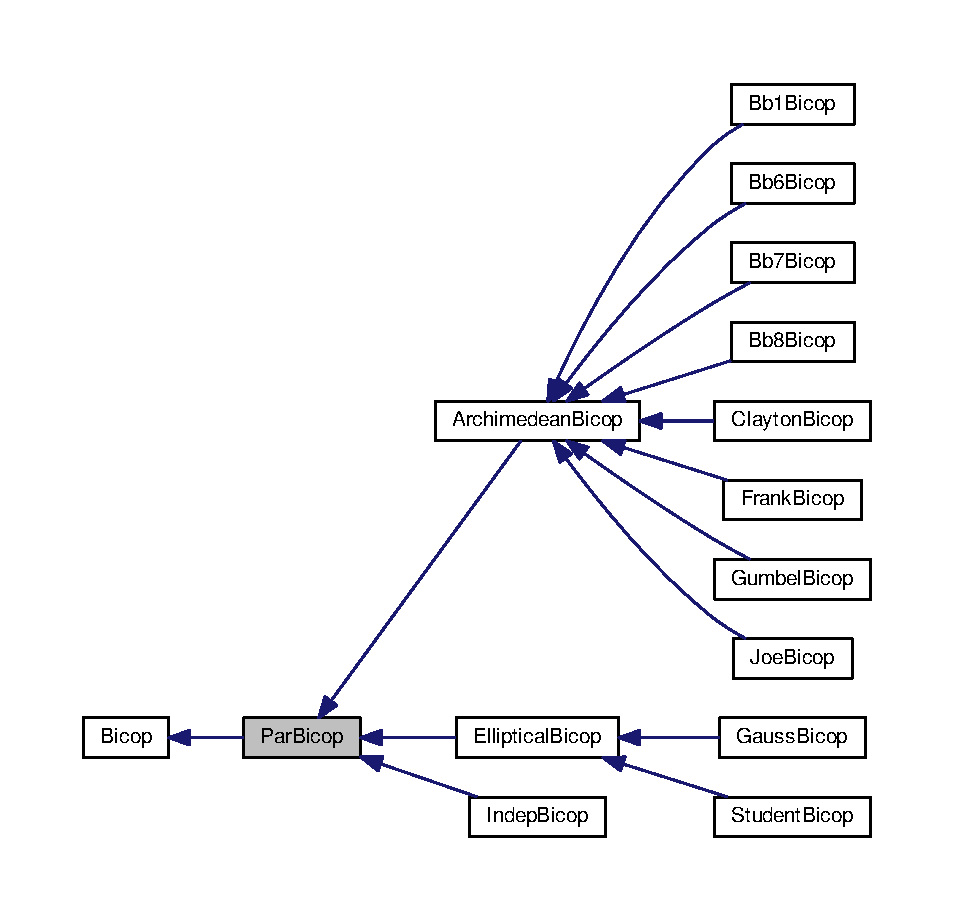
\includegraphics[width=350pt]{class_par_bicop__inherit__graph}
\end{center}
\end{figure}


Collaboration diagram for Par\+Bicop\+:\nopagebreak
\begin{figure}[H]
\begin{center}
\leavevmode
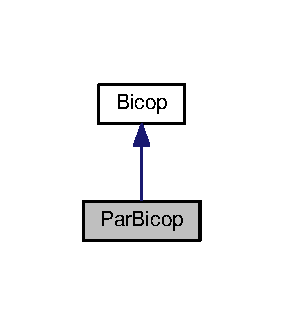
\includegraphics[width=136pt]{class_par_bicop__coll__graph}
\end{center}
\end{figure}
\subsection*{Public Member Functions}
\begin{DoxyCompactItemize}
\item 
void \hyperlink{class_par_bicop_aeab5e7031792bebc04a401a8f135d3a0}{fit} (const Mat\+Xd \&data, std\+::string method)
\item 
virtual double {\bfseries parameters\+\_\+to\+\_\+tau} (const Vec\+Xd \&parameters)=0\hypertarget{class_par_bicop_afa2abb9e5c96798e4c06e79111bb6314}{}\label{class_par_bicop_afa2abb9e5c96798e4c06e79111bb6314}

\item 
double {\bfseries calculate\+\_\+tau} ()\hypertarget{class_par_bicop_af866faf5a92ad12582b50192a033a39c}{}\label{class_par_bicop_af866faf5a92ad12582b50192a033a39c}

\item 
double \hyperlink{class_par_bicop_a190d46ae764f081e2901accade366327}{calculate\+\_\+npars} ()\hypertarget{class_par_bicop_a190d46ae764f081e2901accade366327}{}\label{class_par_bicop_a190d46ae764f081e2901accade366327}

\begin{DoxyCompactList}\small\item\em Get number of parameters. \end{DoxyCompactList}\end{DoxyCompactItemize}
\subsection*{Additional Inherited Members}


\subsection{Member Function Documentation}
\index{Par\+Bicop@{Par\+Bicop}!fit@{fit}}
\index{fit@{fit}!Par\+Bicop@{Par\+Bicop}}
\subsubsection[{\texorpdfstring{fit(const Mat\+Xd \&data, std\+::string method)}{fit(const MatXd &data, std::string method)}}]{\setlength{\rightskip}{0pt plus 5cm}void Par\+Bicop\+::fit (
\begin{DoxyParamCaption}
\item[{const Mat\+Xd \&}]{data, }
\item[{std\+::string}]{method}
\end{DoxyParamCaption}
)\hspace{0.3cm}{\ttfamily [virtual]}}\hypertarget{class_par_bicop_aeab5e7031792bebc04a401a8f135d3a0}{}\label{class_par_bicop_aeab5e7031792bebc04a401a8f135d3a0}
fitstats Fit methods and statistics


\begin{DoxyParams}{Parameters}
{\em u} & $m \times 2$ matrix of observations. \\
\hline
\end{DoxyParams}


Implements \hyperlink{class_bicop_a0ff40d8054e11ed8aaa4956c7fd84e89}{Bicop}.



The documentation for this class was generated from the following files\+:\begin{DoxyCompactItemize}
\item 
/home/n5/dev/cpp/vinecopulib/include/bicop\+\_\+parametric.\+hpp\item 
/home/n5/dev/cpp/vinecopulib/src/bicop\+\_\+parametric.\+cpp\end{DoxyCompactItemize}

\hypertarget{structoptimization__tools_1_1_par_bicop_opt_data}{}\section{optimization\+\_\+tools\+:\+:Par\+Bicop\+Opt\+Data Struct Reference}
\label{structoptimization__tools_1_1_par_bicop_opt_data}\index{optimization\+\_\+tools\+::\+Par\+Bicop\+Opt\+Data@{optimization\+\_\+tools\+::\+Par\+Bicop\+Opt\+Data}}


{\ttfamily \#include $<$optimization\+\_\+tools.\+hpp$>$}



Collaboration diagram for optimization\+\_\+tools\+:\+:Par\+Bicop\+Opt\+Data\+:\nopagebreak
\begin{figure}[H]
\begin{center}
\leavevmode
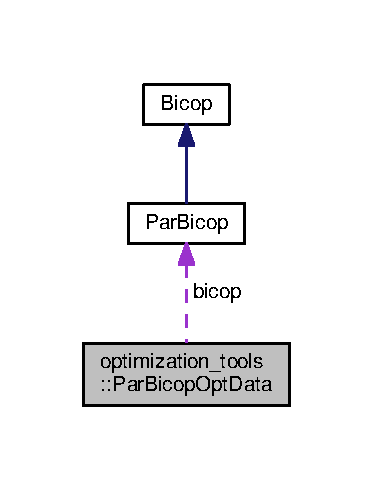
\includegraphics[width=179pt]{structoptimization__tools_1_1_par_bicop_opt_data__coll__graph}
\end{center}
\end{figure}
\subsection*{Public Attributes}
\begin{DoxyCompactItemize}
\item 
const Mat\+Xd \& {\bfseries U}\hypertarget{structoptimization__tools_1_1_par_bicop_opt_data_aac227c20bf1319f39d830d2b1813648d}{}\label{structoptimization__tools_1_1_par_bicop_opt_data_aac227c20bf1319f39d830d2b1813648d}

\item 
\hyperlink{class_par_bicop}{Par\+Bicop} $\ast$ \hyperlink{structoptimization__tools_1_1_par_bicop_opt_data_a9ab9163a5fa571ff992505711ee0d6e9}{bicop}\hypertarget{structoptimization__tools_1_1_par_bicop_opt_data_a9ab9163a5fa571ff992505711ee0d6e9}{}\label{structoptimization__tools_1_1_par_bicop_opt_data_a9ab9163a5fa571ff992505711ee0d6e9}

\begin{DoxyCompactList}\small\item\em The data. \end{DoxyCompactList}\item 
double \hyperlink{structoptimization__tools_1_1_par_bicop_opt_data_ae975b618fc0f6b1c5c17b430b3fdc582}{par0}\hypertarget{structoptimization__tools_1_1_par_bicop_opt_data_ae975b618fc0f6b1c5c17b430b3fdc582}{}\label{structoptimization__tools_1_1_par_bicop_opt_data_ae975b618fc0f6b1c5c17b430b3fdc582}

\begin{DoxyCompactList}\small\item\em A pointer to the bivariate copula to optimize. \end{DoxyCompactList}\item 
unsigned int \hyperlink{structoptimization__tools_1_1_par_bicop_opt_data_a30ba76cb34de8ceb44731469a39bc8bb}{objective\+\_\+calls}\hypertarget{structoptimization__tools_1_1_par_bicop_opt_data_a30ba76cb34de8ceb44731469a39bc8bb}{}\label{structoptimization__tools_1_1_par_bicop_opt_data_a30ba76cb34de8ceb44731469a39bc8bb}

\begin{DoxyCompactList}\small\item\em The main dependence parameter. \end{DoxyCompactList}\end{DoxyCompactItemize}


\subsection{Detailed Description}
A helper struct for nlopt (profile) maximum likelihood estimation 

The documentation for this struct was generated from the following file\+:\begin{DoxyCompactItemize}
\item 
/home/n5/dev/cpp/vinecopulib/include/optimization\+\_\+tools.\+hpp\end{DoxyCompactItemize}

\hypertarget{class_r_vine_matrix}{}\section{R\+Vine\+Matrix Class Reference}
\label{class_r_vine_matrix}\index{R\+Vine\+Matrix@{R\+Vine\+Matrix}}
\subsection*{Public Member Functions}
\begin{DoxyCompactItemize}
\item 
Vec\+Xi {\bfseries get\+\_\+order} ()\hypertarget{class_r_vine_matrix_ab153356e21a86ccdf1e586eade3771b6}{}\label{class_r_vine_matrix_ab153356e21a86ccdf1e586eade3771b6}

\item 
Mat\+Xi \hyperlink{class_r_vine_matrix_aa4c4b6db1e03ca248e6ee2977d94c122}{in\+\_\+natural\+\_\+order} ()
\item 
Mat\+Xi \hyperlink{class_r_vine_matrix_a41f2c2fcfbf6cddb85783d164c26f7cf}{get\+\_\+max\+\_\+matrix} ()
\end{DoxyCompactItemize}
{\bf }\par
\begin{DoxyCompactItemize}
\item 
\hyperlink{class_r_vine_matrix_ab58141cea327509270023fc7ea28fc4a}{R\+Vine\+Matrix} ()
\item 
{\bfseries R\+Vine\+Matrix} (const Mat\+Xi \&matrix)\hypertarget{class_r_vine_matrix_a815d158891d25984bf199b459d77bb3c}{}\label{class_r_vine_matrix_a815d158891d25984bf199b459d77bb3c}

\end{DoxyCompactItemize}

{\bf }\par
\begin{DoxyCompactItemize}
\item 
Mat\+Xi \hyperlink{class_r_vine_matrix_a7ce70c0f0f93f3e42dde78797cce7ebc}{get\+\_\+matrix} ()
\end{DoxyCompactItemize}

{\bf }\par
\begin{DoxyCompactItemize}
\item 
Mat\+Xb \hyperlink{class_r_vine_matrix_a4492de2a5c849a09a48f2aacfa2da553}{get\+\_\+needed\+\_\+hfunc1} ()
\item 
Mat\+Xb {\bfseries get\+\_\+needed\+\_\+hfunc2} ()\hypertarget{class_r_vine_matrix_af986964fb480b66f7ccebde78dc98dfd}{}\label{class_r_vine_matrix_af986964fb480b66f7ccebde78dc98dfd}

\end{DoxyCompactItemize}

\subsection*{Static Public Member Functions}
\begin{DoxyCompactItemize}
\item 
static Mat\+Xi \hyperlink{class_r_vine_matrix_ac18325bf187aa488c79adb5a94fff3ab}{construct\+\_\+d\+\_\+vine\+\_\+matrix} (const Vec\+Xi \&order)
\end{DoxyCompactItemize}


\subsection{Constructor \& Destructor Documentation}
\index{R\+Vine\+Matrix@{R\+Vine\+Matrix}!R\+Vine\+Matrix@{R\+Vine\+Matrix}}
\index{R\+Vine\+Matrix@{R\+Vine\+Matrix}!R\+Vine\+Matrix@{R\+Vine\+Matrix}}
\subsubsection[{\texorpdfstring{R\+Vine\+Matrix()}{RVineMatrix()}}]{\setlength{\rightskip}{0pt plus 5cm}R\+Vine\+Matrix\+::\+R\+Vine\+Matrix (
\begin{DoxyParamCaption}
{}
\end{DoxyParamCaption}
)\hspace{0.3cm}{\ttfamily [inline]}}\hypertarget{class_r_vine_matrix_ab58141cea327509270023fc7ea28fc4a}{}\label{class_r_vine_matrix_ab58141cea327509270023fc7ea28fc4a}
constructors Constructors 

\subsection{Member Function Documentation}
\index{R\+Vine\+Matrix@{R\+Vine\+Matrix}!construct\+\_\+d\+\_\+vine\+\_\+matrix@{construct\+\_\+d\+\_\+vine\+\_\+matrix}}
\index{construct\+\_\+d\+\_\+vine\+\_\+matrix@{construct\+\_\+d\+\_\+vine\+\_\+matrix}!R\+Vine\+Matrix@{R\+Vine\+Matrix}}
\subsubsection[{\texorpdfstring{construct\+\_\+d\+\_\+vine\+\_\+matrix(const Vec\+Xi \&order)}{construct_d_vine_matrix(const VecXi &order)}}]{\setlength{\rightskip}{0pt plus 5cm}Mat\+Xi R\+Vine\+Matrix\+::construct\+\_\+d\+\_\+vine\+\_\+matrix (
\begin{DoxyParamCaption}
\item[{const Vec\+Xi \&}]{order}
\end{DoxyParamCaption}
)\hspace{0.3cm}{\ttfamily [static]}}\hypertarget{class_r_vine_matrix_ac18325bf187aa488c79adb5a94fff3ab}{}\label{class_r_vine_matrix_ac18325bf187aa488c79adb5a94fff3ab}
Construct a D-\/vine matrix

A D-\/vine is a vine where each tree is a path.


\begin{DoxyParams}{Parameters}
{\em order} & order of the variables\\
\hline
\end{DoxyParams}
\begin{DoxyReturn}{Returns}
An Eigen\+::\+Matrix\+Xi describing the D-\/vine structure. 
\end{DoxyReturn}
\index{R\+Vine\+Matrix@{R\+Vine\+Matrix}!get\+\_\+matrix@{get\+\_\+matrix}}
\index{get\+\_\+matrix@{get\+\_\+matrix}!R\+Vine\+Matrix@{R\+Vine\+Matrix}}
\subsubsection[{\texorpdfstring{get\+\_\+matrix()}{get_matrix()}}]{\setlength{\rightskip}{0pt plus 5cm}Mat\+Xi R\+Vine\+Matrix\+::get\+\_\+matrix (
\begin{DoxyParamCaption}
{}
\end{DoxyParamCaption}
)}\hypertarget{class_r_vine_matrix_a7ce70c0f0f93f3e42dde78797cce7ebc}{}\label{class_r_vine_matrix_a7ce70c0f0f93f3e42dde78797cce7ebc}
Getters \index{R\+Vine\+Matrix@{R\+Vine\+Matrix}!get\+\_\+max\+\_\+matrix@{get\+\_\+max\+\_\+matrix}}
\index{get\+\_\+max\+\_\+matrix@{get\+\_\+max\+\_\+matrix}!R\+Vine\+Matrix@{R\+Vine\+Matrix}}
\subsubsection[{\texorpdfstring{get\+\_\+max\+\_\+matrix()}{get_max_matrix()}}]{\setlength{\rightskip}{0pt plus 5cm}Mat\+Xi R\+Vine\+Matrix\+::get\+\_\+max\+\_\+matrix (
\begin{DoxyParamCaption}
{}
\end{DoxyParamCaption}
)}\hypertarget{class_r_vine_matrix_a41f2c2fcfbf6cddb85783d164c26f7cf}{}\label{class_r_vine_matrix_a41f2c2fcfbf6cddb85783d164c26f7cf}
Get maximum matrix

The maximum matrix is derived from an R-\/vine matrix by iteratively computing the (elementwise) maximum of a row and the row below (starting from the bottom). It is used in estimation and evaluation algorithms to find the right pseudo observations for an edge.

no\+\_\+matrix initial R-\/vine matrix, assumed to be in natural order.

\begin{DoxyReturn}{Returns}
An Eigen\+::\+Matrix\+Xi containing the maximum matrix 
\end{DoxyReturn}
\index{R\+Vine\+Matrix@{R\+Vine\+Matrix}!get\+\_\+needed\+\_\+hfunc1@{get\+\_\+needed\+\_\+hfunc1}}
\index{get\+\_\+needed\+\_\+hfunc1@{get\+\_\+needed\+\_\+hfunc1}!R\+Vine\+Matrix@{R\+Vine\+Matrix}}
\subsubsection[{\texorpdfstring{get\+\_\+needed\+\_\+hfunc1()}{get_needed_hfunc1()}}]{\setlength{\rightskip}{0pt plus 5cm}Mat\+Xb R\+Vine\+Matrix\+::get\+\_\+needed\+\_\+hfunc1 (
\begin{DoxyParamCaption}
{}
\end{DoxyParamCaption}
)}\hypertarget{class_r_vine_matrix_a4492de2a5c849a09a48f2aacfa2da553}{}\label{class_r_vine_matrix_a4492de2a5c849a09a48f2aacfa2da553}
Obtain matrix indicating which h-\/functions are needed

It is usually not necessary to apply both h-\/functions for each pair-\/copula.

no\+\_\+matrix initial R-\/vine matrix (assumed to be in natural order).

\begin{DoxyReturn}{Returns}
An Eigen\+::\+Matrix$<$bool, Eigen\+::\+Dynamic, Eigen\+::\+Dynamic$>$ indicating whether hfunc1/2 is needed for a given pair copula. 
\end{DoxyReturn}
\index{R\+Vine\+Matrix@{R\+Vine\+Matrix}!in\+\_\+natural\+\_\+order@{in\+\_\+natural\+\_\+order}}
\index{in\+\_\+natural\+\_\+order@{in\+\_\+natural\+\_\+order}!R\+Vine\+Matrix@{R\+Vine\+Matrix}}
\subsubsection[{\texorpdfstring{in\+\_\+natural\+\_\+order()}{in_natural_order()}}]{\setlength{\rightskip}{0pt plus 5cm}Mat\+Xi R\+Vine\+Matrix\+::in\+\_\+natural\+\_\+order (
\begin{DoxyParamCaption}
{}
\end{DoxyParamCaption}
)}\hypertarget{class_r_vine_matrix_aa4c4b6db1e03ca248e6ee2977d94c122}{}\label{class_r_vine_matrix_aa4c4b6db1e03ca248e6ee2977d94c122}
Reorder R-\/vine matrix to natural order

Natural order means that the diagonal has entries (d, ..., 1). We convert to natural order by relabeling the variables. Most algorithms for estimation and evaluation assume that the matrix is in natural order.

matrix initial R-\/vine matrix.

\begin{DoxyReturn}{Returns}
An Eigen\+::\+Matrix\+Xi containing the matrix in natural order. 
\end{DoxyReturn}


The documentation for this class was generated from the following files\+:\begin{DoxyCompactItemize}
\item 
/home/n5/dev/cpp/vinecopulib/include/rvine\+\_\+matrix.\+hpp\item 
/home/n5/dev/cpp/vinecopulib/src/rvine\+\_\+matrix.\+cpp\end{DoxyCompactItemize}

\hypertarget{class_student_bicop}{\section{Student\+Bicop Class Reference}
\label{class_student_bicop}\index{Student\+Bicop@{Student\+Bicop}}
}


Inheritance diagram for Student\+Bicop\+:
\nopagebreak
\begin{figure}[H]
\begin{center}
\leavevmode
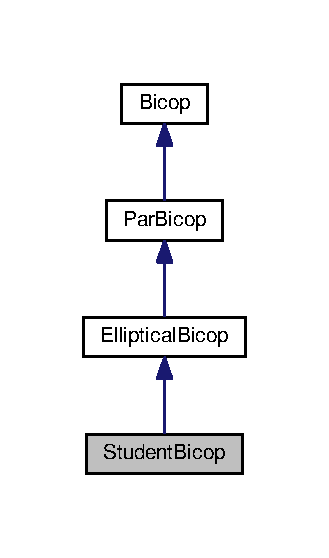
\includegraphics[width=158pt]{class_student_bicop__inherit__graph}
\end{center}
\end{figure}


Collaboration diagram for Student\+Bicop\+:
\nopagebreak
\begin{figure}[H]
\begin{center}
\leavevmode
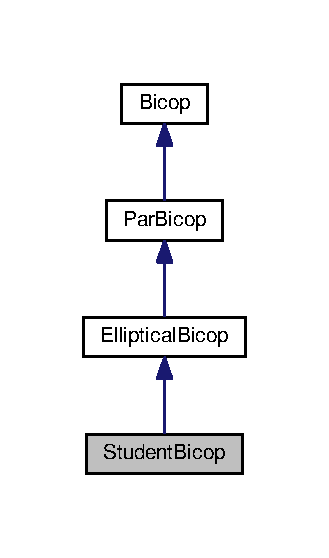
\includegraphics[width=158pt]{class_student_bicop__coll__graph}
\end{center}
\end{figure}
\subsection*{Public Member Functions}
\begin{DoxyCompactItemize}
\item 
\hypertarget{class_student_bicop_af2f1f0ed77021f51e5a148044a677bce}{{\bfseries Student\+Bicop} (double rho, double nu)}\label{class_student_bicop_af2f1f0ed77021f51e5a148044a677bce}

\item 
\hypertarget{class_student_bicop_aa4e65db1840bc768d014468dd8bf9ca8}{Mat\+Xd {\bfseries get\+\_\+bounds} ()}\label{class_student_bicop_aa4e65db1840bc768d014468dd8bf9ca8}

\item 
\hypertarget{class_student_bicop_ab2395bfd3ff086b1d99042fdbb1cbf95}{Vec\+Xd {\bfseries hfunc1} (const Mat\+Xd \&u)}\label{class_student_bicop_ab2395bfd3ff086b1d99042fdbb1cbf95}

\item 
\hypertarget{class_student_bicop_a8d57355f160528f061e974878d4b5deb}{Vec\+Xd {\bfseries hinv1} (const Mat\+Xd \&u)}\label{class_student_bicop_a8d57355f160528f061e974878d4b5deb}

\item 
\hypertarget{class_student_bicop_a83954847188ff122f261f9a35f5971d4}{Vec\+Xd {\bfseries pdf} (const Mat\+Xd \&u)}\label{class_student_bicop_a83954847188ff122f261f9a35f5971d4}

\end{DoxyCompactItemize}
\subsection*{Additional Inherited Members}


The documentation for this class was generated from the following files\+:\begin{DoxyCompactItemize}
\item 
/home/data/uni/\+Promotion/\+Cpp/vinecoplib/src/common/include/bicop\+\_\+student.\+hpp\item 
/home/data/uni/\+Promotion/\+Cpp/vinecoplib/src/common/bicop\+\_\+student.\+cpp\end{DoxyCompactItemize}

\hypertarget{class_trafokernel_bicop}{\section{Trafokernel\+Bicop Class Reference}
\label{class_trafokernel_bicop}\index{Trafokernel\+Bicop@{Trafokernel\+Bicop}}
}


Inheritance diagram for Trafokernel\+Bicop\+:\nopagebreak
\begin{figure}[H]
\begin{center}
\leavevmode
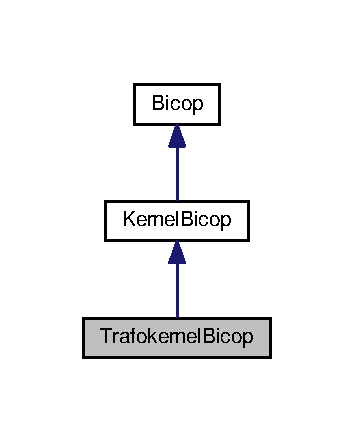
\includegraphics[width=170pt]{class_trafokernel_bicop__inherit__graph}
\end{center}
\end{figure}


Collaboration diagram for Trafokernel\+Bicop\+:\nopagebreak
\begin{figure}[H]
\begin{center}
\leavevmode
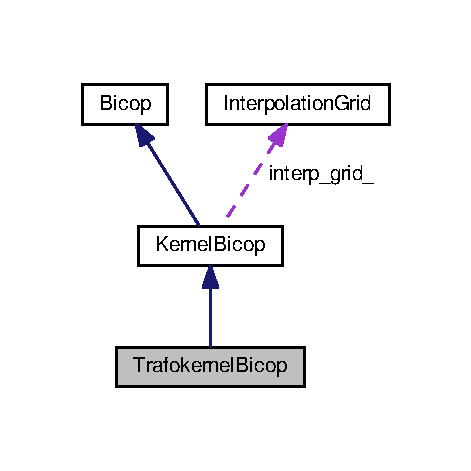
\includegraphics[width=226pt]{class_trafokernel_bicop__coll__graph}
\end{center}
\end{figure}
\subsection*{Public Member Functions}
\begin{DoxyCompactItemize}
\item 
void \hyperlink{class_trafokernel_bicop_ae5da9284cd058b02878614059d8ce078}{fit} (const Mat\+Xd \&data, std\+::string)
\end{DoxyCompactItemize}
\subsection*{Additional Inherited Members}


\subsection{Member Function Documentation}
\hypertarget{class_trafokernel_bicop_ae5da9284cd058b02878614059d8ce078}{\index{Trafokernel\+Bicop@{Trafokernel\+Bicop}!fit@{fit}}
\index{fit@{fit}!Trafokernel\+Bicop@{Trafokernel\+Bicop}}
\subsubsection[{fit}]{\setlength{\rightskip}{0pt plus 5cm}void Trafokernel\+Bicop\+::fit (
\begin{DoxyParamCaption}
\item[{const Mat\+Xd \&}]{data, }
\item[{std\+::string}]{method}
\end{DoxyParamCaption}
)\hspace{0.3cm}{\ttfamily [virtual]}}}\label{class_trafokernel_bicop_ae5da9284cd058b02878614059d8ce078}
fitstats Fit methods and statistics


\begin{DoxyParams}{Parameters}
{\em u} & $m \times 2$ matrix of observations. \\
\hline
\end{DoxyParams}


Implements \hyperlink{class_bicop_a0ff40d8054e11ed8aaa4956c7fd84e89}{Bicop}.


\hypertarget{structstructselect__tools_1_1_vertex_properties}{\section{structselect\+\_\+tools\+:\+:Vertex\+Properties Struct Reference}
\label{structstructselect__tools_1_1_vertex_properties}\index{structselect\+\_\+tools\+::\+Vertex\+Properties@{structselect\+\_\+tools\+::\+Vertex\+Properties}}
}
\subsection*{Public Attributes}
\begin{DoxyCompactItemize}
\item 
\hypertarget{structstructselect__tools_1_1_vertex_properties_ae98731fd772dc856678430a58c89a59c}{std\+::vector$<$ int $>$ {\bfseries conditioning}}\label{structstructselect__tools_1_1_vertex_properties_ae98731fd772dc856678430a58c89a59c}

\item 
\hypertarget{structstructselect__tools_1_1_vertex_properties_a55e4762ff80a2764ad3108296461f1eb}{std\+::vector$<$ int $>$ {\bfseries conditioned}}\label{structstructselect__tools_1_1_vertex_properties_a55e4762ff80a2764ad3108296461f1eb}

\item 
\hypertarget{structstructselect__tools_1_1_vertex_properties_a4417fead3115618173f27aa82dc2a892}{std\+::vector$<$ int $>$ {\bfseries prev\+\_\+edge\+\_\+indices}}\label{structstructselect__tools_1_1_vertex_properties_a4417fead3115618173f27aa82dc2a892}

\item 
\hypertarget{structstructselect__tools_1_1_vertex_properties_a02eb01c5bac207cda84e1bb774af31e0}{Vec\+Xd {\bfseries hfunc1}}\label{structstructselect__tools_1_1_vertex_properties_a02eb01c5bac207cda84e1bb774af31e0}

\item 
\hypertarget{structstructselect__tools_1_1_vertex_properties_a4944630229999934498193b125540b72}{Vec\+Xd {\bfseries hfunc2}}\label{structstructselect__tools_1_1_vertex_properties_a4944630229999934498193b125540b72}

\end{DoxyCompactItemize}

\hypertarget{class_vinecop}{}\section{Vinecop Class Reference}
\label{class_vinecop}\index{Vinecop@{Vinecop}}


A class for vine copulas.  




{\ttfamily \#include $<$vinecop\+\_\+class.\+hpp$>$}

\subsection*{Public Member Functions}
\begin{DoxyCompactItemize}
\item 
\hyperlink{class_vinecop_ac2b043db375e4127234c066ba3b2412e}{Vinecop} (int d)
\item 
\hyperlink{class_vinecop_af7b728d1bc489c6c87e6afb31e82ac06}{Vinecop} (const std\+::vector$<$ std\+::vector$<$ Bicop\+Ptr $>$$>$ \&pair\+\_\+copulas, const Mat\+Xi \&matrix)
\item 
Bicop\+Ptr {\bfseries get\+\_\+pair\+\_\+copula} (int tree, int edge)\hypertarget{class_vinecop_abd9dec1c010eec23f75ee0c8e52384bd}{}\label{class_vinecop_abd9dec1c010eec23f75ee0c8e52384bd}

\item 
int {\bfseries get\+\_\+family} (int tree, int edge)\hypertarget{class_vinecop_a30c95180a72665208e146a4202dcf3d9}{}\label{class_vinecop_a30c95180a72665208e146a4202dcf3d9}

\item 
Mat\+Xi {\bfseries get\+\_\+families} ()\hypertarget{class_vinecop_ae2c34ebbdd6cf388559829de790a3c9c}{}\label{class_vinecop_ae2c34ebbdd6cf388559829de790a3c9c}

\item 
int {\bfseries get\+\_\+rotation} (int tree, int edge)\hypertarget{class_vinecop_a8c2d5cc23ce33027d4024a4d7702e854}{}\label{class_vinecop_a8c2d5cc23ce33027d4024a4d7702e854}

\item 
Mat\+Xi {\bfseries get\+\_\+rotations} ()\hypertarget{class_vinecop_ad71c803ec5f5966a2cde7c14493e4644}{}\label{class_vinecop_ad71c803ec5f5966a2cde7c14493e4644}

\item 
Vec\+Xd {\bfseries get\+\_\+parameters} (int tree, int edge)\hypertarget{class_vinecop_ae0b65eba272c6a2868d1db9f04e1fdbf}{}\label{class_vinecop_ae0b65eba272c6a2868d1db9f04e1fdbf}

\item 
Mat\+Xi {\bfseries get\+\_\+matrix} ()\hypertarget{class_vinecop_aa1c2dcb66503749a66f40f2031d99e0b}{}\label{class_vinecop_aa1c2dcb66503749a66f40f2031d99e0b}

\item 
Vec\+Xd {\bfseries pdf} (const Mat\+Xd \&u)\hypertarget{class_vinecop_af7cc5932cd21a4c8b07805ad79911a4f}{}\label{class_vinecop_af7cc5932cd21a4c8b07805ad79911a4f}

\item 
Mat\+Xd {\bfseries simulate} (int n)\hypertarget{class_vinecop_a2a234b3fdfd00e67cf27b5f3deb09873}{}\label{class_vinecop_a2a234b3fdfd00e67cf27b5f3deb09873}

\item 
Mat\+Xd {\bfseries simulate} (int n, const Mat\+Xd \&U)\hypertarget{class_vinecop_a46ab3b783c58fdaa342c17812590d74b}{}\label{class_vinecop_a46ab3b783c58fdaa342c17812590d74b}

\end{DoxyCompactItemize}
\subsection*{Static Public Member Functions}
\begin{DoxyCompactItemize}
\item 
static std\+::vector$<$ std\+::vector$<$ Bicop\+Ptr $>$ $>$ \hyperlink{class_vinecop_a91167c08796a946141e228f87e01b284}{make\+\_\+pair\+\_\+copula\+\_\+store} (int d)
\item 
static \hyperlink{class_vinecop}{Vinecop} \hyperlink{class_vinecop_a40e56d021bbb4f4d462110e6a9039913}{select} (const Mat\+Xd \&data, std\+::vector$<$ int $>$ family\+\_\+set=\{0, 1, 2, 3, 4, 5, 6, 1001\}, std\+::string method=\char`\"{}mle\char`\"{}, int truncation\+\_\+level=std\+::numeric\+\_\+limits$<$ int $>$\+::max(), Mat\+Xi matrix=Mat\+Xi(0, 0), std\+::string selection\+\_\+criterion=\char`\"{}bic\char`\"{}, bool preselect\+\_\+families=true, bool show\+\_\+trace=false)
\end{DoxyCompactItemize}


\subsection{Detailed Description}
A class for vine copulas. 

\subsection{Constructor \& Destructor Documentation}
\index{Vinecop@{Vinecop}!Vinecop@{Vinecop}}
\index{Vinecop@{Vinecop}!Vinecop@{Vinecop}}
\subsubsection[{\texorpdfstring{Vinecop(int d)}{Vinecop(int d)}}]{\setlength{\rightskip}{0pt plus 5cm}Vinecop\+::\+Vinecop (
\begin{DoxyParamCaption}
\item[{int}]{d}
\end{DoxyParamCaption}
)}\hypertarget{class_vinecop_ac2b043db375e4127234c066ba3b2412e}{}\label{class_vinecop_ac2b043db375e4127234c066ba3b2412e}
Construct a vine copula object of dimension d


\begin{DoxyParams}{Parameters}
{\em d} & dimension of the vine copula.\\
\hline
\end{DoxyParams}
\begin{DoxyReturn}{Returns}
a d-\/dimensional D-\/vine with variable order 1, ..., d and all pair-\/copulas set to independence 
\end{DoxyReturn}
\index{Vinecop@{Vinecop}!Vinecop@{Vinecop}}
\index{Vinecop@{Vinecop}!Vinecop@{Vinecop}}
\subsubsection[{\texorpdfstring{Vinecop(const std\+::vector$<$ std\+::vector$<$ Bicop\+Ptr $>$$>$ \&pair\+\_\+copulas, const Mat\+Xi \&matrix)}{Vinecop(const std::vector< std::vector< BicopPtr >> &pair_copulas, const MatXi &matrix)}}]{\setlength{\rightskip}{0pt plus 5cm}Vinecop\+::\+Vinecop (
\begin{DoxyParamCaption}
\item[{const std\+::vector$<$ std\+::vector$<$ Bicop\+Ptr $>$$>$ \&}]{pair\+\_\+copulas, }
\item[{const Mat\+Xi \&}]{matrix}
\end{DoxyParamCaption}
)}\hypertarget{class_vinecop_af7b728d1bc489c6c87e6afb31e82ac06}{}\label{class_vinecop_af7b728d1bc489c6c87e6afb31e82ac06}
Construct a vine copula object from a vector$<$\+Bicop\+Ptr$>$ and structure matrix


\begin{DoxyParams}{Parameters}
{\em pair\+\_\+copulas} & a nested vector of Bicop\+Ptrs; can be initialized by make\+\_\+pair\+\_\+copula\+\_\+store(d). \\
\hline
{\em matrix} & R-\/vine matrix.\\
\hline
\end{DoxyParams}
\begin{DoxyReturn}{Returns}
a d-\/dimensional D-\/vine with variable order 1, ..., d and all pair-\/copulas set to independence 
\end{DoxyReturn}


\subsection{Member Function Documentation}
\index{Vinecop@{Vinecop}!make\+\_\+pair\+\_\+copula\+\_\+store@{make\+\_\+pair\+\_\+copula\+\_\+store}}
\index{make\+\_\+pair\+\_\+copula\+\_\+store@{make\+\_\+pair\+\_\+copula\+\_\+store}!Vinecop@{Vinecop}}
\subsubsection[{\texorpdfstring{make\+\_\+pair\+\_\+copula\+\_\+store(int d)}{make_pair_copula_store(int d)}}]{\setlength{\rightskip}{0pt plus 5cm}std\+::vector$<$ std\+::vector$<$ Bicop\+Ptr $>$ $>$ Vinecop\+::make\+\_\+pair\+\_\+copula\+\_\+store (
\begin{DoxyParamCaption}
\item[{int}]{d}
\end{DoxyParamCaption}
)\hspace{0.3cm}{\ttfamily [static]}}\hypertarget{class_vinecop_a91167c08796a946141e228f87e01b284}{}\label{class_vinecop_a91167c08796a946141e228f87e01b284}
Initialize object for storing pair copulas


\begin{DoxyParams}{Parameters}
{\em d} & dimension of the vine copula. \\
\hline
\end{DoxyParams}
\begin{DoxyReturn}{Returns}
A nested vector such that pc\+\_\+store(d)\mbox{[}t\mbox{]}\mbox{[}e\mbox{]} contains a Bicop\+Ptr to the pair copula corresponding to tree t and edge e. 
\end{DoxyReturn}
\index{Vinecop@{Vinecop}!select@{select}}
\index{select@{select}!Vinecop@{Vinecop}}
\subsubsection[{\texorpdfstring{select(const Mat\+Xd \&data, std\+::vector$<$ int $>$ family\+\_\+set=\lcurly{}0, 1, 2, 3, 4, 5, 6, 1001\rcurly{}, std\+::string method=""mle"", int truncation\+\_\+level=std\+::numeric\+\_\+limits$<$ int $>$\+::max(), Mat\+Xi matrix=\+Mat\+Xi(0, 0), std\+::string selection\+\_\+criterion=""bic"", bool preselect\+\_\+families=true, bool show\+\_\+trace=false)}{select(const MatXd &data, std::vector< int > family_set=\{0, 1, 2, 3, 4, 5, 6, 1001\}, std::string method="mle", int truncation_level=std::numeric_limits< int >::max(), MatXi matrix=MatXi(0, 0), std::string selection_criterion="bic", bool preselect_families=true, bool show_trace=false)}}]{\setlength{\rightskip}{0pt plus 5cm}{\bf Vinecop} Vinecop\+::select (
\begin{DoxyParamCaption}
\item[{const Mat\+Xd \&}]{data, }
\item[{std\+::vector$<$ int $>$}]{family\+\_\+set = {\ttfamily \{0,~1,~2,~3,~4,~5,~6,~1001\}}, }
\item[{std\+::string}]{method = {\ttfamily \char`\"{}mle\char`\"{}}, }
\item[{int}]{truncation\+\_\+level = {\ttfamily std\+:\+:numeric\+\_\+limits$<$int$>$\+:\+:max()}, }
\item[{Mat\+Xi}]{matrix = {\ttfamily MatXi(0,~0)}, }
\item[{std\+::string}]{selection\+\_\+criterion = {\ttfamily \char`\"{}bic\char`\"{}}, }
\item[{bool}]{preselect\+\_\+families = {\ttfamily true}, }
\item[{bool}]{show\+\_\+trace = {\ttfamily false}}
\end{DoxyParamCaption}
)\hspace{0.3cm}{\ttfamily [static]}}\hypertarget{class_vinecop_a40e56d021bbb4f4d462110e6a9039913}{}\label{class_vinecop_a40e56d021bbb4f4d462110e6a9039913}
Automated model and structure selection for vine copulas

Implements the structure selection algorithm of Dissmann et al. (2013).


\begin{DoxyParams}{Parameters}
{\em data} & nxd matrix of copula data. \\
\hline
{\em family\+\_\+set} & the set of copula families to consider (if empty, then all families are included; all families are included by default). \\
\hline
{\em method} & indicates the estimation method\+: either maximum likelihood estimation (method = \char`\"{}mle\char`\"{}, default) or inversion of Kendall\textquotesingle{}s tau (method = \char`\"{}itau\char`\"{}). When method = \char`\"{}itau\char`\"{} is used with families having more thanone parameter, the main dependence parameter is found by inverting the Kendall\textquotesingle{}s tau and the remainders by profile likelihood optimization. \\
\hline
{\em selection\+\_\+criterion} & the selection criterion; either \char`\"{}aic\char`\"{} or \char`\"{}bic\char`\"{} (default). \\
\hline
{\em preselect\+\_\+families} & whether to exclude families before fitting based on symmetry properties of the data. \\
\hline
{\em show\+\_\+trace} & whether to show a trace of the building progress (default is false). \\
\hline
\end{DoxyParams}
\begin{DoxyReturn}{Returns}
The fitted vine copula model. 
\end{DoxyReturn}


The documentation for this class was generated from the following files\+:\begin{DoxyCompactItemize}
\item 
/home/n5/dev/cpp/vinecopulib/include/vinecop\+\_\+class.\+hpp\item 
/home/n5/dev/cpp/vinecopulib/src/vinecop\+\_\+class.\+cpp\end{DoxyCompactItemize}

\chapter{File Documentation}
\hypertarget{mainpage_8h}{}\section{/home/n5/dev/cpp/vinecopulib/include/mainpage.h File Reference}
\label{mainpage_8h}\index{/home/n5/dev/cpp/vinecopulib/include/mainpage.\+h@{/home/n5/dev/cpp/vinecopulib/include/mainpage.\+h}}


api\+\_\+docs  




\subsection{Detailed Description}
api\+\_\+docs 


%--- End generated contents ---

% Index
\backmatter
\newpage
\phantomsection
\clearemptydoublepage
\addcontentsline{toc}{chapter}{Index}
\printindex

\end{document}
